% This file contains CHAPTER FIVE

\chapter{Explicit Formulas for Genus 2 Arithmetic}\label{cha:g2} 
In this chapter, derivations of explicit formulas for genus 2 hyperelliptic
curves given by a ramified and split model are described. 
%Tables describing explicit formulas for doubling and addition in the frequent 
%cases are presented in Appendix~\ref{app:g2RAM} for ramified models and 
%Appendix~\ref{app:g2SPLIT} for split models. 
All explicit formulas presented in this chapter are
implemented in Magma along with implementations of random input testing and
automatic generation of inputs that cover every output case. Automated
operation counting and latex table generation scripts were also developed to
circumvent errors in the operation count and explicit formula presentations. All
software developed for this thesis is available at
\url{https://github.com/salindne/divisorArithmetic}.


\section{Improved Genus 2 Ramified Model Explicit Formulas}
\label{sec:g2ramExpl}
In this section, novel explicit formulas for addition and doubling of divisor
classes on genus 2 hyperelliptic curve ramified models are described. In
general, the curve equation of a ramified model for a genus 2 hyperelliptic
curve in Weierstrass form is $C: y^2 + h(x)y = f(x)$ where
$$f = x^5 + f_4x^4 + f_3x^3 + f_2 x^2 + f_1x + f_0, \s\s\s\s\s h = h_2x^2 + h_1x
+ h_0$$ with $h_2 \in \{1,0\}$. Curve coefficients are represented as vectors of
field elements $$f = [f_4,f_3,f_2,f_1,f_0], \s\s\s h = [h_2,h_1,h_0].$$ Input
and output divisors are represented as 4-coordinate vectors of field elements $$
D = [u_1,u_0,v_1,v_0],$$ for the Mumford representation $D = [u,v]$ with $u =
x^2 + u_1x + u_0$ and $v = v_1x + v_0$. Only 4 coordinates are required, the
least number of coordinates possible resulting in formulas that are the
simplest.

The improvements in this work are obtained by working from versions of NUCOMP
and NUDUPL specialized to genus 2 (Algorithms~\ref{alg:g2nucomp}
and~\ref{alg:g2nudupl}) and combining the best ideas from prior works. The
formulas are complete in the sense that all possible input and output cases are
given explicitly as opposed to falling back on Cantor's algorithm when special
cases arise. In all underlying field considerations, arbitrary, char($k) = 2$
and char($k) \not = 2$ fields, this yields novel formulas requiring fewer field
operations than any others to date. Moreover,  all explicit formulas presented
require only one inversion through any computation path, including all special
cases. 

This section is structured as follows. First, assumptions about curve models
over certain fields are discussed, then an overview of prior work is provided.
This is followed by a statement of the novel contributions in this work and then
a description of the basic formulations for doubling and addition are provided.
Finally, operation costs in terms of field operations, comparisons to
previous work, and empirical benchmarking results are presented.

\subsection{Curve Simplifications} 
\label{sect:curvesimplifications} 
The efficiency of explicit formulas somewhat depends on the equation of the
hyperelliptic curve as the polynomial-based algorithms for divisor class
arithmetic presented in the previous chapters involve computations with $f$ and
$h$. Isomorphic models of the curve with more zero coefficients in $f$ and $h$
allow for explicit formulas with fewer field operations. Assumptions and
simplifications to the hyperelliptic equation of a curve are discussed, starting
with curve isomorphisms that transform a ramified model curve into another
isomorphic ramified model curve with a less complex
equation~\cite{HandbookHECC_2006}. 

Recall that a ramified model for a genus 2 hyperelliptic curve can be given as
$$C : y^2 + h(x)y = f(x) $$ where $h(x)$ is at most degree two, and $f(x)$ is at
most degree five. An isomorphic transformation of $C$ is defined as a
transformation of the variables $x$ and $y$ (change of variables) to other
expressions involving $x$ and $y$; see~\cite{HandbookHECC_2006}. What isomorphic
transformations can be applied depends on the characteristic of the underlying
field the curve is defined over. Next, the isomorphic transformations that are
possible over fields of characteristic two and characteristic not equal to two are
described; for more details see~\cite{Lange_explicit_2005}. 

\subsubsection{char(k) $\neq$ 2}
If char($k$) $\neq$ 2, then applying the substitution $y \rightarrow y - h(x)/2$
invokes the transformation 
\begin{align*}
y^2 + h(x)y = f(x) &\rightarrow (y-h(x)/2)^2 + h(x)(y - h(x)/2) = f(x) \\
                   &\implies y^2 -2h(x)y/2 + (h(x))^2/4 + h(x)y -2(h(x))^2/4 = f(x) \\
                   &\implies y^2 = f'(x)
\end{align*} 
where $f' = f + (h(x))^2/2$. This transformation is always possible when
char($k) \neq 2$, allowing the assumption of $h=0$ in this case. If the
characteristic of the underlying field is also not five, the transformation $ x
\rightarrow x - f_4/5 $ that takes $f(x) \rightarrow f(x)'$ to get $$ f(x)' =
x^5 + f_3'x^3 + f_2'x^2 + f_1'x + f_0'$$ can be applied, allowing one to assume
that $f_4 = 0$ in that case. Operation counts in Section~\ref{sec:ramFieldCosts}
assume $h = 0$ whenever char($k) \neq 2$, but make no assumption about $f_4$.

\subsubsection{char(k) = 2}
If char($k$) = 2, then division by two is not
possible and the transformation $$ y \rightarrow y - \frac{h(x)}{2}$$ cannot be
made. In the genus 2 setting $h$ non-constant is guaranteed because otherwise
the curve model is singular. The following isomorphism transforms a curve to
one for which several coefficients of $h$ and $f$ are zero or one: $$ y
\rightarrow h_2^5y + f_3h_2x + \frac{f_3(f_3 + h_1h_2 + f_4h_2^2 +
f_2h_2^2)}{h_2^3}, \quad x\rightarrow h_2^2x + f_4.$$ Dividing the equation by
$h_2^{10}$ results in $h_2 =1$ and $f_4 = f_3 = f_2 = 0$. This equation of the curve
is assumed when counting operations in Section~\ref{sec:ramFieldCosts} over
base field $k$ with char($k) = 2$. 

\subsection{Prior Work}
\label{sec:g2explRAMPriorWork}
Most prior work mentioned in this section only applies to divisor class
arithmetic over fields with char($k) \not = 2$, where isomorphisms can be
applied to ensure that $h(x) = 0$. The work of this thesis not only improves on
divisor class arithmetic in that setting, but also extends to arbitrary base
fields where no assumptions about the equation of the curve are made,  as well as
specializations to the case char($k) = 2$.

In~\cite{Lange_explicit_2005}, Lange presented affine explicit formulas over
fields with char($k) = 2$ and char($k) \not = 2$ using 4 coordinate
representation $(u_1,u_0,v_1,v_0)$. Each coordinate in the representation is a coefficient of
a polynomial in Mumford representation (Section~\ref{sec:mumford}) for
generic genus 2 curves with a ramified model in Weierstrass form. Frequent cases
and some special cases where the output degree in the frequent case is less than
the genus, as well as adding degree one with degree two divisors are presented.
The novel work of this thesis directly improves on this prior work.

The author also gave a description for computing all other special cases. Some
suggestions do not work in all settings, for example suggestion 2b)ii) on page
7 of~\cite[Section~4.1]{Lange_explicit_2005} results in an infinite loop if the
divisor class being composed has 3 torsion. Most of the suggestions required
several inversions as presented. More details are provided in
Sections~\ref{sec:g2RAMDBL} and~\ref{sec:g2RAMADD}.

In~\cite{CostelloLauter_geo_2011}, the authors presented $6$-coordinate affine
formulas for adding and doubling divisor classes in the frequent cases only
based on the linear algebra method (Section~\ref{sec:geometric}) that applies a
system of linear equations in the composition portion of Cantor's Algorithm. The
extra coordinates are $U_0 = u_0u_1$ and $U_1=u_1^2$, which are computed at the
end of each operation, but also required in the beginning of the next operation.
To avoid computing the same values twice in chains of operations, $U_0$ and
$U_1$ are passed as auxiliary coordinates. Numerical testing in Magma on a
consistent platform presented in Section~\ref{sec:g2numerical} suggests that
although the field multiplication or squaring counts are smaller, as shown in
Table~\ref{tab:ramfcosts}, a surplus of field additions results in explicit
formulas that perform worse than not only the formulas of this work but in some
cases also those of~\cite{Lange_explicit_2005}.

\subsection{Contributions Summary}
\label{sec:g2explRAMOurContr}
This work provides complete explicit formulas, in the sense that all computation
paths are explicitly computed, requiring only one inversion in all cases that
take reduced divisor class representatives as input, and output a reduced
divisor class representative. Not only is every special case explicitly
computed, this work also improves on previous best in the frequent cases of
addition and doubling. 
%Frequent case explicit formulas are given in Appendix~\ref{app:g2RAM}. 
All formulas are implemented in Magma including a
testing suite (described in Section~\ref{sec:g2numerical}) to ensure their
correctness. The implemented formulas and testing scripts are available at
\url{https://github.com/salindne/divisorArithmetic}.

The formulations of divisor class addition and doubling are based on NUCOMP
specialized to genus 2 addition and doubling that includes efficient
formulations of special cases. The formulation of steps in
Algorithms~\ref{alg:g2nucomp} and~\ref{alg:g2nudupl}, coupled with certain
explicit techniques produce the fastest explicit formulas for frequent case
addition and doubling to date. The formulas incorporate different techniques
borrowed from previous works and also introduce a new technique presented in
Section~\ref{sec:vsave}. 

A summary of the novel techniques that differ from previous work is as follows:
\begin{enumerate}[label=T\arabic*]
\item \label{tq:1} 
Use a system of equations~\cite{Balamohan_MSc_2009,CostelloLauter_geo_2011} to
solve for $s=s_1x + s_0$ rather than computing the resultant as done by Harley
and others (see Section~\ref{sec:alternateharley}). In contrast, the linear
algebra method uses a system of equations to directly solve for $V = su_1 + v_1$.
\item \label{tq:2} 
Compute the coefficients of the output $u$ and $v$ polynomials using a NUCOMP
based polynomial formulation specialized to genus 2. This technique allows for
the reuse of computations from solving for $s$ through the system of equations.
\item \label{tq:3} 
Compute $v$ differently by omitting the direct computation of $su_1$ and use
$s,u_1$ directly as described in Section~\ref{sec:vsave}.
\item \label{tq:4} Include explicit one inversion formulas via the specialized
NUCOMP formulations (Algorithms~\ref{alg:g2nucomp} and~\ref{alg:g2nudupl})
for all special cases with $\gcd (u_1,u_2,v_1 + v_2 + h) \not = 1$ producing
vastly more efficient formulas for special cases when compared to previous
suggestions~\cite{Lange_explicit_2005}.
\end{enumerate}

Note that in this work, the equating coefficient technique for computing the
output Mumford polynomial $u$ from~\cite{CostelloLauter_geo_2011} (described in
Section~\ref{sec:equatingcoeff}) produced identical formulations for computing
$u$ when compared to a direct computation of $u$ via NUCOMP as in Addition and
Doubling Algorithms~\ref{alg:g2nucomp} and~\ref{alg:g2nudupl}. Moreover, the
threshold for trading field multiplications for field additions is capped at 1
multiplication for 3 additions throughout (see Section~\ref{sec:trades}.)

\subsubsection{Special Cases}
All implementations of frequent case arithmetic include explicit handling of
special cases as they come up naturally in the computations via
Technique~\ref{tq:4}. All computation paths through special cases in the
formulas require only one inversion. The formulations are based on
Algorithm~\ref{alg:g2nucomp}, that includes efficient handling of special cases
at the level of polynomial arithmetic, see Section~\ref{sec:nucompbasis}.
Compared to the formulas of this work, the suggestions from previous
work~\cite{Lange_explicit_2005} on handling these cases produced far more
cumbersome explicit formulas, between 20 and 40 percent more field
operations. The reduction in the number of field operations can be
attributed to the removal of algorithms requiring lower degree input polynomials with weighted
inputs, as required when implementing one inversion versions of the special case
suggestions from~\cite{Lange_explicit_2005}. 


\subsection{Explicit Formulas for Doubling}
\label{sec:g2RAMDBL} 
In this section, complete divisor class doubling is described and the basic
formulations of the corresponding explicit formulas are provided. Doubling
Algorithm~\ref{alg:g2nudupl} is further specialized to different cases
depending on the input divisor class degree. The explicit techniques used are
discussed in each case. 

The complete doubling algorithm should test the degree of the input divisor
class representative in order of statistical frequency, calling degree 2
doubling (Algorithm~\ref{alg:explRAM2DBL}) and degree 1 doubling
(Algorithm~\ref{alg:explRAM1DBL}) accordingly. The neutral element is returned
if the degree of the input divisor class representative is zero, and therefore
the neutral element itself.  In the following, the basic formulations required
for complete doubling, organized by the degree of the input divisor are
provided.

\subsubsection{Genus 2 Ramified Model Degree 2 Doubling}
Let $[u_1,v_1]$ be a reduced divisor class representative with $u_1 = x^2 +
u_{11}x + u_{10}$ and $v_1 = v_{11}x + v_{10}$. Steps~1-5 in
Algorithm~\ref{alg:g2nudupl} are specialized to degree 2 doubling by
computing the resultant $d = \mathrm{Res}(u_1,2v_1+h)$ instead of $S =
\mathrm{XGCD}(u_1,2v_1 + h)$ in Step~2 of Algorithm~\ref{alg:g2nudupl}, where
$d=0$ implies $S \neq 1$. In this case $b_1 = 1/(2v_1 + h) \pmod{u_1}$ so $s
= k/(h + 2v_1) \pmod{u_1}$ in Step~5 of Doubling Algorithm~\ref{alg:g2nudupl}.
The resultant $d$ is computed by first setting up a system of equations to solve
for the coefficients of $s$ via the equality $s(h + 2v_1) = k \pmod{u_1}$, for
which the determinant of the resulting 2x2 matrix with coefficients $m_i$ is the
resultant $d$ (see Section~\ref{sec:alternateharley}).

The computation of the $k$ polynomial in Step~1 of Algorithm~\ref{alg:g2nudupl}
is postponed until after the computation of $d$, and instead $d$ is immediately
checked for special cases. If $d \neq 0$, then there are no common factors
between $u_1$ and $2v_1 + h$, and Steps~5 and~9--11 of Doubling
Algorithm~\ref{alg:g2nudupl} are executed. Steps~8-9 of Doubling
Algorithm~\ref{alg:g2nudupl} are combined in all output cases taking advantage
of combining terms that need to be multiplied by precomputed weights to make
$u_n$ monic. If $d = 0$, then Steps~4,5,7 are performed instead, described in
Subroutine~\ref{sub:explRAM2DBLd}. 

The basic formulation for degree 2 doubling, adapted from Doubling
Algorithm~\ref{alg:g2nudupl}, is described in Algorithm~\ref{alg:explRAM2DBL}.
An explanation of how each step in Algorithm~\ref{alg:explRAM2DBL} is converted
to an explicit formula is given in the following.

\begin{algorithm}[htbp]
\caption{Genus 2 Ramified Model Degree 2 Doubling\label{alg:explRAM2DBL}}
\begin{algorithmic}[1]
\Require $[D_1] = [u_1,v_1]$, $f$, $h$.  \smallskip
\Ensure $[u_n,v_n] = 2[D_1]$.
\algrule
\State Compute $m_i$ in system for $s(h + 2v_1) = k' \pmod{u_1}$ as $ \bigl[
\begin{smallmatrix} m_4 & -m_2\\ -m_3 & m_1\end{smallmatrix}\bigr] \bigl[
\begin{smallmatrix} s_0\\ s_1 \end{smallmatrix} \bigr ] = \bigl[ \begin{smallmatrix}k'_0
\\  k'_1\end{smallmatrix} \bigr ]$.
\State $d = m_1m_4 - m_2m_3$.
\If{$d$ is 0} Go to Subroutine~\ref{sub:explRAM2DBLd}.
\EndIf
\State $k' = (f - v_1(v_1 + h))/u_1 \pmod{u_1}. \s\s\s$ (and $k = (f - v_1(v_1 + h))/u_1$)
\State Solve for $s_1' = ds_1, s_0' = ds_0$ using the $m_i$ and Cramer's rule, omitting the inversion of $d$.
\If{$s_1' =  0$}
    \State $s_0 = s_0'/d$.
    \State $u_n = -(s_0(2v_1 + h) - k)/u_1 - s_0^2 \s\s\s $ (exact division).
    \State $v_n = (-s_0u_1 - v_1 - h) \pmod{u_n}$.
    \State \Return $[u_n,v_n]$.
    \EndIf
\State $w = 1/(ds_1')$ and precompute values $1/s_1$, $1/s_1^2$ and $s_1$. 
\State Compute monic $s'' = x + s_0''$ where $s_0'' = s_0'/s_1'$.
\State $u_n = (s'')^2 + (s''(2v_1 + h) - k/s_1)/(s_1u_1) \s\s\s $ (exact division, made monic).
\State $v_n = (-s_1s''u_1 - v_1 - h) \pmod{u_n}$.
\State \Return $[u_n,v_n]$.
\end{algorithmic}
\end{algorithm}


In Step 1, the polynomial representation $$ k'_1x + k'_0 =
(\vt_1x + \vt_0)(s_1x + s_0) - s_1\vt_1(x^2 + u_{11}x + u_{10})$$ is used to
solve for $s_1,s_0$ where $$s = s_1x + s_0 = (k'_1x + k'_0)/(\vt_1x + \vt_0)
\pmod{x^2 + u_{11}x + u_{10}}$$ and $\vt = 2v_1 + h \pmod{u_1}$. By equating
coefficients, the following equations linear in coefficients of $s$ arise:  
\begin{align*} k'_0 &=
(\vt_0) \cdot s_0 + (-\vt_1u_{10}) \cdot s_1, \\
k'_1 &= (\vt_1) \cdot s_0 + (\vt_0 - \vt_1u_{11}) \cdot s_1.
\end{align*}
Consider the following $2 \times 2$ system $$ \left( \begin{array}{cc}
\vt_0 & -\vt_1u_{10}   \\
\vt_1 & \vt_0 -\vt_1u_{11}   \end{array} \right) \times \left( \begin{array}{c}
s_0   \\
s_1   \end{array} \right) = \left( \begin{array}{c}
k'_0   \\
k'_1   \end{array} \right), $$  representing the identities above. Instead 
set up the system  as $$ \left( \begin{array}{cc}
m_4 & -m_2   \\
-m_3 & m_1   \end{array} \right) \times \left( \begin{array}{c}
s_0   \\
s_1   \end{array} \right) = \left( \begin{array}{c}
k'_0   \\
k'_1   \end{array} \right),$$ for $m_4 = \vt_0, m_2 = \vt_1u_{10}, m_3 = -\vt_1,
m_1 = -\vt_1u_{11}$. Multiplying both sides by the inverse of the the matrix
yields the following expressions for $s_1$ and $s_0$ $$ \left( \begin{array}{cc}
m_1/d & m_2/d   \\
m_3/d & m_4/d   \end{array} \right) \times \left( \begin{array}{c}
k'_0   \\
k'_1   \end{array} \right) = \left( \begin{array}{c}
s_0   \\
s_1   \end{array} \right),$$ where the $d$ is the determinant.
The resulting explicit formula for the $m_i$ in Step~1 and $d$ in Step~2 is 
\begin{align*}
    \vh_0 &= v_{10} + h_0, \\
    \vh_1 &= v_{11} + h_1,\\
    m_3 &= h_2u_{11} - v_{11} - \vh_1,\\
    m_4 &= v_{10} + \vh_0 - h_2u_{10},\\ 
    m_1 &= m_4 + m_3u_{11},\\
    m_2 &= -m_3u_{10}, \\
    d &= m_1m_4 - m_2m_3,
\end{align*} with $\vh_1$ and $\vh_0$ reused later in the computation of output
polynomials $u_n$ and $v_n$.

If $d \neq 0$, then in Step~4 the polynomial $$k' = k'_1x + k'_0 = (f- hv_1 -
v_1^2)/u_1 \pmod{u_1}$$ is computed. First the exact division by $u_1$ is
computed, then the modular reduction of the result by $u_1$ collecting
expressions for the coefficients of $k'_1$ and $k'_0$. The resulting explicit
formula for Step~4 is
\begin{align*}
    t_0 &= u_{11}^2,\\
    t_1 &= f_3 + t_0 - h_2v_{11},\\
    t_2 &= u_{10} + u_{10},\\
    t_3 &= f_4u_{11},\\
    t_4 &= f_4u_{10},\\
    t_5 &= t_0 - t_3,\\
    t_6 &= t_1 - t_2,\\
    k_1 &= t_5 + t_5 + t_6,\\
    k_0 &= u_{11}(t_2 - t_6 + t_3) + f_2 - v_{11}\vh_1 - t_4 - t_4 - h_2v_{10}.
\end{align*}

In Step~5, the solution of the system of equations $s' = sd$ given by the
resulting 2x2 matrix after inversion above is computed (see
Section~\ref{sec:alternateharley}), where the resulting explicit formula is
\begin{align*}
s_0' &= k'_0m_1 + k'_1m_2\\
s_1' &= k'_0m_3 + k'_1m_4.
\end{align*}
    
If $s_1' = 0$ the special output case is invoked with $\deg(s') = 0$. The value
$s_0 = s_0'/d$ is computed directly in Step~7, followed by $u = s^2 + (s(2v_1 +
h) - k)/u_1$ and $v = (-su_1 - v_1 - h) \pmod{u}$ in Steps~8-9. Notice that
since $\deg(k) = 3$, with $k = (f - v_1(v_1 + h))/u_1$, where coefficients $k_3
= 1, k_2 = f_4 - u_{11}$, the resulting $u_n'$ (not normalized) is $u_n' = -x +
s_0h_2 - f_4 + 2u_1 + s_0^2.$ Normalization results in $u_n = x + u_{n_0}$ with
$$u_{n_0} = f_4 - s_0^2 - s_0h_2 - 2u_{11}.$$ The polynomial $v_n$ is computed
via a direct school book modular reduction of the polynomial $$-s_0u_1 - v_1 - h
= -(s_0 + h_2)x^2 - (s_0u_{11} + h_1)x - (s_0u_{10} + h_0)$$ by $x + u_{n_0}$,
resulting in the explicit formulation
\begin{align*} 
    t_1     &= s_0(u_{11} - u_{n_0}) - h_2^2u_{n_0} + \vh_1,\\
    v_{n_0} &= u_{n_0}t_1 - \vh_0 - s_0u_{10}.    
\end{align*} 
The field multiplication pattern for Karatsuba reduction does not occur
(Section~\ref{sec:karatsubared}).

If $s_1' \neq 0$ then in Steps~11--12 the required weights for normalizing $u_n$, along with
$s_1$ and monic $s'' = x + s_0''$ for $s_0'' = s_0/s_1$ are computed. The
resulting explicit formula (with the actual
values given in brackets) is
\begin{align*} 
    w_1 &= (ds_1')^{-1},\\
    w_2 &= w_1d, \s\s\s\s\s\s\s (1/(ds_1))\\
    w_3 &= w_2d, \s\s\s\s\s\s\s (1/s_1)\\
    w_4 &= w_3^2, \s\s\s\s\s\s\s\s\s (1/(s_1^2))\\
    s_1 &= w_1(s_1')^2,\\
    s_0'' &= s_0'w_2, \end{align*} as described in Section~\ref{sec:reordering}. 

In Step~13, the polynomial $u_n' = s^2 + (s(2v_1 + h) - k)/u_1$ requires a
division by $s_1^2$ to be normalized, so 
$$ u_n = (s'')^2 + ((s''(2v_1+ h) - k/s_1)/u_1)/s_1$$ is computed, utilizing an
exact division (see Section~\ref{sec:exactdiv}). The resulting explicit formula
for Step~13 is 
\begin{align*}
    t_2 &= s_0''- w_4 + h_2w_3,\\
    u_{n_1} &= s_0'' + t_2,\\
    u_{n_0} &= (s_0'')^2 + w_3(h_2(s_0'' - u_{11}) + v_{11} + \vh_1) + w_4(2u_{11} - f_4),
\end{align*}
with $k$ as described above. 

In Step~14, the polynomial $v_n = (-s_1s''u_1 - v_1 - h) = (-su_1 - v_1 - h)
\pmod{u_n}$ is computed. School book modular reduction is applied instead of
Karatsuba to take advantage of reusing sub-expressions. Applying a school book
modular reduction results in
\begin{align*}
    v_{n_1} &= s_1(u_1s_0''+ u_1u_{11} - u_{n_1}^2 - s_0''u_{11}
    + u_{n_0} - u_{10}) - v_{11} - h_1 + h_2u_1\\
            &= s_1((u_{n_1} - s_0'')(u_{11} - u_{n_1}) + u_{n_0} - u_{10}) - v_{11} - h_1 + h_2u_1\\
    v_{n_0} &= s_1(u_0s_0'' + u_{11}u_{n_0} - u_0u_1 -s_0''u_{10}) - v_{10} - h_0 + h_2u_0\\
            &= s_1(s_0''(u_{n_0} - u_{10}) + u_{n_0}(u_{11} - u_{n_1})) - v_{10} - h_0 + h_2u_0.
\end{align*} 
Recall that in Step~13, $u_{n_1} = s_0'' + t_2$ and so $t_2 = u_{n_1} - s_0''$.
This combined with the formula for Step~14 above results in the following
explicit formula for Step~14: 
\begin{align*}  
    t_0 &= u_{n_0} - u_{10},\\
    t_1 &= u_{11} - u_{n_1},\\
    v_{n_1} &= s_1(t_2t_1 + t_0) - v_{11} - h_1 + h_2u_1\\
    v_{n_0} &= s_1(s_0''t_0 + u_{n_0}t_1) - v_{10} - h_0 + h_2u_0,
\end{align*}
as described in Section~\ref{sec:vsave}. 

For $d=0$ and $\deg(S) = 2$, with $S$ from Doubling
Algorithm~\ref{alg:g2nudupl}, the input divisor class representative $[u_1,v_1]$
has order 2, resulting in the output of the neutral divisor class. Otherwise,
exactly one point with $x$-coordinate determined by $S = x - m_4/m_3$ (one of the two factors of
$u_1$) has two torsion. The polynomial $S$ is removed from $u_1$ via an exact
division (Section~\ref{sec:exactdiv}). The basic formulation of the case $d = 0$
within degree 2 doubling is presented in Subroutine~\ref{sub:explRAM2DBLd}. An
explanation of how each step in Subroutine~\ref{sub:explRAM2DBLd} is converted
to an explicit formula is given in the following. 

\begin{subroutine}[htbp]
\caption{Genus 2 Ramified Model Degree 2 Doubling ($d = 0$) \label{sub:explRAM2DBLd}}
\begin{algorithmic}[1]
\State Let $d_w = (h + 2v_1) \pmod{u_1} -m_3x + m_4.$
\If{$m_3$ is 0} \hspace{1pt} \Return $[1,0]$.
\EndIf
\State $k = (f - v_1(v_1 + h))/u_1$.
\State $b_1 = 1/$lcf$(d_w) \s\s\s$ (made monic).
\State $u_1 = b_1u_1/d_w$.
\State $s = b_1k \pmod{u_1}$.
\State $u_n = u_1^2$
\State $v_n = (v_1 + u_1s) \pmod{u_n}$.
\State \Return $[u_n,v_n]$.
\end{algorithmic}
\end{subroutine}

Step~1, reuses the computations of $m_3$ and $m_4$ from  degree 2 doubling
Algorithm~\ref{alg:explRAM2DBL}, resulting in $d_w = -m_3x + m_4$. In Step~3 ,
an exact division by the original input $u_1$ polynomial is computed in $k = (f
- v_1(v_1 + h))/u_1$ . The resulting explicit formula for Step~3 is 
\begin{align*}
    k_2 &= f_4 - u_{11},\\
    k_1 &= f_3 - v_{11}h_2 - u_{10} - u_{11}k_2,\\
    k_0 &= f_2 - v_{11}\vh_1 - v_{10}h_2 - u_{10}k_2 - u_{11}k_1.
\end{align*} In Steps~4--5, the leading coefficient $-m_3$ of $d_w$ is inverted and $u_1$
divided by monic $d_w$. The explicit formula for Steps~4--5 is $$b_1 =
-m_3^{-1}, \s\s\s\s\s\s u_{10} = u_{11} - m_4b_1.$$ In Steps~6--8, the
polynomial $s = b_1k \pmod{u_1}$ is computed by a modular reduction, $u_n =
u_1^2$ by a polynomial squaring and $v_n = (v_1 + u_1s_0) \pmod{u_n}$ by a
modular reduction as well. Since $\deg(u_1) = 1$, the multiplication pattern
required for Karatsuba reduction (Section~\ref{sec:karatsubared}) does not arise
and therefore school book reductions are applied.  The resulting explicit
formula for Steps~6-8 is
\begin{align*}
    s_0 &= b_1(k_0 - u_{10}(k_1 - u_{10}(k_2 - u_{10}))),\\
u_{n_1} &= u_{10} + u_{10},\\
u_{n_0} &= u_{10}^2,\\
v_{n_1} &= v_{11} + s_0,\\
v_{n_0} &= v_{10} + s_0u_{10}.    
\end{align*}


\subsubsection{Genus 2 Ramified Model Degree 1 Doubling}
Let $[u_1,v_1]$ be a reduced divisor class representative with $u_1 = x +
u_{10}$ and $v_1 = v_{10}$.  Degree 1 doubling is computed by Steps~1-7 of
Doubling Algorithm~\ref{alg:g2nudupl}. The resultant $d =
\mathrm{Res}(u_1,2v_1+h)$ is computed instead of $S = \mathrm{XGCD}(u_1,2v_1 +
h)$ in Step~2 of Algorithm~\ref{alg:g2nudupl}, where $d=0$ implies $S \neq 1$.
In this case, $b_1 = 1/(2v_1 + h) \pmod{u_1}$ and so $s = k/(h + 2v_1)
\pmod{u_1}$ in Step~5 of Doubling Algorithm~\ref{alg:g2nudupl}. The basic
formulation for degree 1 doubling is described in
Algorithm~\ref{alg:explRAM1DBL}. An explanation of how each step in
Algorithm~\ref{alg:explRAM1DBL} is converted to an explicit formula is given in
the following.

\begin{algorithm}[htbp]
\caption{Genus 2 Ramified Model Degree 1 Doubling\label{alg:explRAM1DBL}}
\begin{algorithmic} [1]
\Require $[D_1] = [u_1,v_1]$, $f$, $h$.  \smallskip
\Ensure $[u_n,v_n] = 2[D_1]$.
\algrule
\State $d = (h + 2v_1) \pmod{u_1}$.
\If{$d$ is 0} \Return $[1,0]$.
\EndIf
\State $k' = (f - v_1(v_1 + h))/u_1 \pmod{u_1}$.
\State $s_0 = k'/d \pmod{u_1} \s\s$ where $1/d = b_1$.
\State $u_n = u_1^2$.
\State $v_n = s_0u_1 + v_1  \pmod{u_n}.$
\State \Return $[u_n,v_n]$.
\end{algorithmic}
\end{algorithm}

In Step~1, the resultant $d = (h + 2v_1) \pmod{u_1}$ is computed by a school
book modular reduction, since $\deg(u_1) = 1$. The equality $d = 0$ is
immediately checked in Step~2, and if so, the appropriate special case invoked
where the single $x$-coordinate represented by $u$ corresponding to the affine
point in the divisor class has two torsion and the neutral element is returned.
Steps~3--5 are performed similarly to Steps~6--8 of Degree 2 Doubling when $d=0$ using
Subroutine~\ref{sub:explRAM2DBLd}.


\subsection{Explicit Formulas for Addition}\label{sec:g2RAMADD}
In this section, complete divisor class addition is described and the basic
formulations of the corresponding explicit formulas are provided. Addition
Algorithm~\ref{alg:g2nucomp} is further specialized to different cases
depending on the input divisor class degree. The explicit techniques used are
discussed in each case. 

The complete addition algorithm should test the degree of the input divisor
class in order of statistical frequency, calling degree 2 addition
(Algorithm~\ref{alg:explRAM2ADD}), degree 1 with 2 addition
(Algorithm~\ref{alg:explRAM12ADD}) and degree 1 addition
(Algorithm~\ref{alg:explRAM1ADD}) accordingly. The neutral element is returned
if the degree of both input divisor classes is zero.  In the following, the
basic formulations required for complete addition, organized by the degree of
the input divisor class are provided.

\subsubsection{Genus 2 Ramified Model Degree 2 Addition}
Let $[u_1,v_1]$ and $[u_2,v_2]$ be reduced divisor class representatives with
$u_1 = x^2 + u_{11}x + u_{10}$, $v_1 = v_{11}x + v_{10}$ and $u_2 = x^2 +
u_{21}x + u_{20}$, $v_2 = v_{21}x + v_{20}$. Steps~1-11 in
Algorithm~\ref{alg:g2nucomp} are specialized to degree 2 addition by computing
the resultant $d = \mathrm{Res}(u_1,u_2)$ instead of $S = \mathrm{XGCD}(u_1
u_2)$ in Step~2 of Algorithm~\ref{alg:g2nucomp}, where $d=0$ implies $S
\neq 1$. In this case $a_1 = 1/u_1 \pmod{u_2}$ so $s = (v_2 - v_1)/u_1
\pmod{u_2}$ in Step~11 of Addition Algorithm~\ref{alg:g2nucomp}. The resultant
$d$ is computed by first setting up a system of equations to solve for the
coefficients of $s$ via the equality $su_1 = (v_2 - v_1) \pmod{u_2}$, for which the
determinant of the resulting 2x2 matrix with coefficients $m_i$ is the resultant
$d$ (see Section~\ref{sec:alternateharley}).

The computation of the $k$ polynomial in Step~1 of Algorithm~\ref{alg:g2nucomp}
is postponed until after the computation of $d$, and instead $d$ is immediately
checked for special cases. If $d \neq 0$, then there are no common factors
between $u_1$ and $u_2$, and Steps~11,15--19 of Addition
Algorithm~\ref{alg:g2nucomp} are performed. Steps~15-16 of Addition
Algorithm~\ref{alg:g2nucomp} are combined in all output cases taking advantage
of combining terms that need to be multiplied by precomputed weights to make
$u_n$ monic. If $d = 0$, then a check for $d_w = \mathrm{Res}(u_1,v_2 + v_1 + h)
= 0$ is made, and if true, the appropriate points are removed. If $d_w \neq
0$, then $s$ is computed by Step~9 of Addition Algorithm~\ref{alg:g2nucomp},
described in Subroutine~\ref{sub:explRAM2ADDd}. 

The basic formulation for degree 2 addition, adapted from Addition
Algorithm~\ref{alg:g2nucomp}, is described in Algorithm~\ref{alg:explRAM2ADD}.
An explanation of how each step in Algorithm~\ref{alg:explRAM2ADD} is converted
to an explicit formula is given in the following.


\begin{algorithm}[htbp]
\caption{Genus 2 Ramified Model Degree 2 Addition\label{alg:explRAM2ADD}}
\begin{algorithmic}[1]
\Require $[D_1] = [u_1,v_1]$, $[D_2] = [u_2,v_2]$, $[D1] \not = [D2]$ \smallskip
\Ensure $[u_n,v_n] = [D_1] + [D_2] $.
\algrule
\vspace{-3pt}
\State Compute $m_i$ in system of equations for $su_1\equiv \vt \pmod{u_2}$ as $ \bigl[ \begin{smallmatrix} m_4 & -m_2\\ -m_3 & m_1\end{smallmatrix}\bigr] \bigl[ \begin{smallmatrix} s_0\\ s_1 \end{smallmatrix} \bigr ] = \bigl[ \begin{smallmatrix}\vt_0 \\  \vt_1\end{smallmatrix} \bigr ]$, where $\vt = \vt_1x + \vt_0 = v_2 - v_1$.
\State $d = m_1m_4 - m_2m_3$.
\If{$d = 0$} \hspace{1pt} Go to Degree 2 Addition $d=0$ Subroutine~\ref{sub:explRAM2ADDd}.
\EndIf
\State Solve for $s_1' = ds_1, s_0' = ds_0$ using the $m_i$ and Cramer's rule, omitting the inversion of $d$.
\If{$s_1' =  0$}
    \State $s_0 = s_0'/d$.
    \State $\vt = -s_0u_1 - v_1 - h$.
    \State $k = (f - v_1(v_1 + h))/u_1 \pmod{u_1}$.
    \State $u_n = (s_0(\vt - v_1) + k)/u_2 \s\s\s$ (exact division).
    \State $v_n = \vt \pmod{u_n}$.
    \State \Return $[u_n,v_n]$.
\EndIf
\State $w = 1/(ds_1')$ and precompute the values $1/s_1, 1/(s_1)^2, s_1$. 
\State Compute monic $s'' = x + s_0''$ where $s_0'' = s_0'/s_1'$.
\State $k = (f - v_1(v_1 + h))/u_1$.
\State $\vt = -su_1 - v_1 - h$.
\State $u_n = (s''(\vt - v_1/s_1) + k/s_1^2)/u_2 \s\s\s$ (exact division).
\State $v_n = \vt \pmod{u_n}$.
\State \Return $[u_n,v_n]$.
\end{algorithmic}
\end{algorithm}


In Step~1, a similar computation to Degree 2 Doubling (Algorithm~\ref{alg:explRAM2DBL}) for
the matrix coefficients $m_i$ and $d$ is performed using the system of equations 
\begin{align*} 
    \vt_0 &= (u_{10} - u_{20}) \cdot s_0 + (u_{20}(u_{21} - u_{10})) \cdot s_1,\\
    \vt_1 &= -(u_{21}- u_{11}) \cdot s_0 + (u_{10} - u_{20} + u_{21}(u_{21}-u_{11})) \cdot s_1,
\end{align*} linear in $s_1$ and $s_0$, for $s = (v_2 - v_1)/u_1 \pmod{u_2}$.

If $d \neq 0$, then in Step~4, the solution of the system of equations $s' = sd$
is computed (Section~\ref{sec:alternateharley}), where the explicit formula
for Step~4 is
\begin{align*}
    \vt_1 &= v_{21} - v_{11},\\
    \vt_0 &= v_{20} - v_{10},\\
    s_0' &= \vt_0m_1 + \vt_1m_2,\\
    s_1' &= \vt_0m_3 + \vt_1m_4.
\end{align*}

If $s_1' = 0$ the special output case is invoked with $\deg(s') = 0$. The value
$s_0 = s_0'/d$ is computed followed a direct computation of Steps~15--17 of
Addition Algorithm~\ref{alg:g2nucomp} where $\vt = -su_1 - v_1 - h$ is
combined into $u_n =(s(\vt - v_1) + k)/u_2$ and $v_n = \vt \pmod{u_n}$ is
computed directly. Since $\deg(k) = 3$ with coefficients $k_3 = 1, k_2 = f_4 -
u_{11}$, the direct compuation of output polynomial $u_n$ is already monic and
$$u_n = x + f_4 - u_{11} - u_{21} - s_0^2 - h_2s_0$$ by an exact division (see
Section~\ref{sec:exactdiv}). The polynomial $v_n$
is computed via a school book modular reduction of the polynomial $$-s_0u_1 - v_1 - h =
-(s_0 + h_2)x^2 - (s_0u_{11} + h_1)x - (s_0u_{10} + h_0)$$ by the polynomial $x
+ u_{n_0}$, resulting in
\begin{align*} t_1 &= s_0(u_{11} - u_{n_0}) - h_2^2u_{n_0} + v_{11} + h_1,\\
v_{n_0} &= u_{n_0}t_1 - \vh_0 - s_0u_{10}.    
\end{align*}

If $s_1' \neq 0$ then in Steps~12--13 the required weights for normalizing
$u_n$, along with $s_1$ and monic $s'' = x + s_0''$ for $s_0'' = s_0/s_1$, are
computed. The resulting explicit formula for Steps~12--13 is 
\begin{align*} 
    w_1 &= (ds_1')^{-1},\\
    w_2 &= w_1d, \s\s\s\s\s\s\s (1/(ds_1))\\
    w_3 &= w_2d, \s\s\s\s\s\s\s (1/(s_1))\\
    w_4 &= w_3^2, \s\s\s\s\s\s\s (1/(s_1)^2)\\
    s_1 &= w_1(s_1')^2,\\
    s_0'' &= s_0'w_2,
\end{align*} as described in Section~\ref{sec:reordering}.

In Steps~14--16, the polynomial $u_n' = (s(-su_1 - 2v_1 - h ) + k)/u_2$ requires a division by $s_1^2$ to
be normalized, so $$ u_n = s''(\vt - v_1/s_1) + k/(s_1)^2)/u_2$$ is computed combining the three steps,
utilizing an exact division (see Section~\ref{sec:exactdiv}), and taking advantage
of combining terms that need to be multiplied by the precomputed weights $w_i$.
The resulting formula for Steps~14--16 is 
\begin{align*}
    t_3 &= s''_0 - m_3,\\
    t_2 &= t_3- w_4 + h_2w_3,\\
    \vh_1 &= h_1 + v_1,\\
    u_{n_1} &= s_0'' + t_2,\\
    u_{n_0} &= s_0''(t_3 - m_3) + m_1 + w_3(h_2(s''_0 - u_{21}) + \vh_1 + v_{11}) + w_4(u_{11} + u_{21} - f_4),
\end{align*}
where only the degree $2$ coefficient $k_2 = $ of $k$ is used. In Step~17,
computation of the polynomial $v_n = \vt \equiv (-su_1 - v_1 - h) \pmod{u_n}$ is
identical to degree 2 doubling (also see Section~\ref{sec:vsave}.)

The basic formulation of the case $d = 0$ within degree 2 addition is presented
as Subroutine~\ref{sub:explRAM2ADDd}. An explanation of how each step in
Subroutine~\ref{sub:explRAM2ADDd} is converted to an explicit formula is given
in the following. 

\begin{subroutine}[htbp]
    \caption{Genus 2 Ramified Model Degree 2 Addition ($d=0$)\label{sub:explRAM2ADDd}}
    \begin{algorithmic}[1]
    \State Let and $d_{w_1} = u_1 \pmod{u_2} = -m_3x + m_4$.
    \If{$m_3$ is 0} 
        \State $d_{w_2} = (v_2 + v_1 + h) \pmod{u_1}$.
        \If{$d_{w_2}$ is 0} \Return $[1,0]$.
        \Else 
            \State $k = (f - v_1(v_1 + h))/u_1 \pmod{u_1}$.
            \State $d_{w_2}$ = $\monic(d_{w_2})$ with $b_2 = 1/$lcf$(d_{w_2})$.
            \State $u_1 = u_1/d_{w_2}$
            \State $s = b_2k \pmod{u_1}$.
            \State $u_n = u_1^2$.
            \State $v_n = (v_1 + su_1) \pmod{u_n}$.
            \State \Return $[u_n,v_n]$.
        \EndIf
    \Else 
        \State Compute weighted $d_{w_3} = (v_2 + v_1 + h) \pmod{d_{w_1}}$.
        \If{$d_{w_3}$ is 0}
            \State $u_c = \monic(d_{w_1})$ with $a_1 = 1/$lcf$(d_{w_1})$.
            \State $u_1 = u_1/d_{w_1}$.
            \State $s = a_1(v_2 - v_1) \pmod{u_2}$.
            \State $u_n = u_1u_2$.
            \State $v_n = (v_1 + su_1) \pmod{u_n}$.
            \State \Return $[u_n,v_n]$.
        \Else 
            \State $k = (f - v_1(v_1 + h))/u_1 \pmod{u_1}$.
            \State $a_{12} = a_1(1 - b_2(v_1 + v_2 + h))/d_{w_1} \pmod{u_2}$ with weight $m_3d_{w_3}$
            \State $s' = s_1'x + s_0' = d_{w_3}s_1x + d_{w_3}s_0 = (a_{12}(v_2 - v_1) + m_3^3k) \pmod{u_2}$, with weight $d_{w_3}$.
            \State Go to Step~5 of Degree 2 Addition Algorithm~\ref{alg:explRAM2ADD}, with $d = d_{w_3}$.
        \EndIf
    \EndIf
    \end{algorithmic}
    \end{subroutine}


In the case $d = 0$, there exists at least one common $x$-coordinate among the
two input divisor classes. With $d=0$, if $\gcd(u_1,u_2) = u_1$ (equivalently
$m_3 = 0$) and assuming $[D_1] \not = [D_2]$, then for Steps~3-12, there are two
possible cases: either all four points being compared are opposite, or two are
opposite and two are common, (since all four points being common implies a
doubling scenario.) If the divisor classes contain all opposites, then $v_1 =
(-v_2 -h) \pmod{u_1}$ and equivalently $d_{w_2} = (v_2 + v_1 + h) \pmod{u_1} =
0$, resulting in a return of the neutral divisor class. Otherwise the opposite
point is extracted through an exact division by $\monic(d_{w_2})$ and computed
similarly as in Subroutine~\ref{sub:explRAM2DBLd}.

With $d=0$, if $m_3 \neq 0$, and equivalently $\gcd(u_1,u_2) \neq u_1$, then
only one point computed via $\gcd(u_1,u_2)$, is common or opposite. In
Steps~14--15, $d_{w_3} = (v_2 + v_1 + h) \pmod{d_{w_1}}$ is computed to check
for the existence of an opposite point. If $d_{w_3} = 0$, then in Steps~16--17
the opposite point is extracted through an exact division by $u_c =
\monic(d_{w_1})$ and computed similarly to the special degree 2 doubling case,
but two degree 1 divisors are added. In Step~18, the polynomial $s = a_1(v_2 -
v_1) \pmod{u_2}$ is computed via a school book modular reduction and
Steps~19--20 compute $u_n = u_1u_2$ and $v_n = (v_1 + u_1s_0) \pmod{u_n}$  via a
school book polynomial multiplication and modular reduction respectively. 

Otherwise for Steps~23--25, $d_{w_3} \neq 0$ and  a weighted $s' = s_1'x + _0'$
is computed as $s = (a_2a_1(v_2 - v_1) + b_2k) \pmod{u_2}$, omitting the
inversion required for $a_1 = 1/-m_3$. First
$$a_{12} = -a_1a_2 = m_3^2(h_2u_{21) - v_{21} - t_1})$$ where $a_2 = (1 -
b_2(v_1 + v_2 + h) \pmod{u_2})/\monic(d_{w_1})$ is computed with weight
$m_3d_{w_3}$. Then the $k_2,k_1,k_0$ coefficients of $k = (f - v_1(v_1 +
h)/u_1)$ are computed as described in degree 2 ramified doubling. Finally, $s =
a_2a_1(v_2 - v_1)+ b_2k) \pmod{u_2}$ is computed using the above values. The
explicit formula for Steps~23--25 is
\begin{align*}
    a_{12} &= M_3(h_2u_{21} - v_{21} - t_1),\\   
    t_2 &= k_2 - u_{21},\\
    t_0 &= m_3M_3,\\
    s_1' &= t_0(k_1 - u_{20} - u_{21}t_2) - a_{12}(v_{21} - v_{11}),\\
    s_0' &= t_0(k_0 - u_{20}t_2) - a_{12}(v_{20} - v_{10}),\\
    d_1 &= m_3d_{w_3},
\end{align*} with $t_1 = v_{11} + h_1$ and $M_3 = m_3^2$ computed earlier. The 
rest of the computations are identical to the frequent case of degree 2 addition
starting at Step~5 of Algorithm~\ref{alg:explRAM2ADD} with $d = d_{w_3}$.

\subsubsection{Genus 2 Ramified Model Degree 1 and 2 Addition}
Let $[u_1,v_1]$ and $[u_2,v_2]$ be reduced divisor class representatives with
$u_1 = x^2 + u_{11}x + u_{10}$, $v_1 = v_{11}x + v_{10}$ and $u_2 = x + u_{20}$,
$v_2 = v_{20}$. Algorithm~\ref{alg:g2nucomp}  is specialized to
degree 1 and 2 addition by computing the resultant $d = \mathrm{Res}(u_1,u_2)$
instead of $S = \mathrm{XGCD}(u_1 u_2)$ in Step~2 of
Algorithm~\ref{alg:g2nucomp}, where $d=0$ implies $S \neq 1$. In this case $a_1
= 1/u_1 \pmod{u_2}$ and so $s = (v_2 - v_1)/u_1 \pmod{u_2}$ in Step~11 of
Addition Algorithm~\ref{alg:g2nucomp}. The computation of $k$ in Step~1 of
Algorithm~\ref{alg:g2nucomp} is not required in all cases and is pushed further
into the algorithm. The basic formulation for degree 1 and 2 addition is
described in Algorithm~\ref{alg:explRAM12ADD}. An explanation of how each step
in Algorithm~\ref{alg:explRAM12ADD} is converted to an explicit formula is given
in the following.

\begin{algorithm}[htbp]
\caption{Genus 2 Ramified Model Degree 1 and 2 Addition\label{alg:explRAM12ADD}}
\begin{algorithmic} [1]
\Require $[D_1] = $ degree 2 $[u_1,v_1]$, $[D_2] = $ degree 1 $ [u_2,v_2]$, \smallskip
\Ensure $[u_n,v_n] = [D_1] + [D_2] $.
\algrule
\State $d = u_1 \pmod{u_2}$.
\If{$d$ is 0} \hspace{1pt} Go to Degree 1 and 2 Addition $d=0$ Subroutine~\ref{sub:explRAM12ADDd}.
\EndIf
\State $a_1 = d^{-1}$.
\State $s_0 = a_1(v_2 - v_1) \pmod{u_2}$.
\State $k = ((f - v_1(v_1 + h))/u_1) \pmod{u_1}$.
\State $\vt = -s_0u_1 - v_1 - h$.
\State $u_n = (s_0(\vt - v_1) + k)/u_2 \s\s\s$ (exact division).
\State $v_n = \vt \pmod{u_n}$.
\State \Return $[u_n,v_n]$.
\end{algorithmic}
\end{algorithm}

In Step~1, the resultant $d = u_1 \pmod{u_2}$ is computed via a school book
modular reduction with a degree one modulus. If $d \neq 0$, then in Steps~3--4
$s = s_0 = a_1(v_2 - v_1) \pmod{u_2}$ is computed via a school book modular
reduction and an inversion $a_1 = 1/d$. In Step~5, the polynomial $k$ is monic
and has degree 3 and the polynomial $\vt$ has degree 2. Only the degree one and two
coefficients of $k$ and $\vt$ are required in the computation of $u_n$, where
the computation of $\vt$ and $u_n$ are combined and computed via an exact
division in Steps~6--7. In this case, the output $u_n$ polynomial computed is
already monic, since $k$ is monic. In Step~8 $v_n$ is computed via a school book
modular reduction of a degree 2 polynomial modulo a degree 2 polynomial where
the Karatsuba multiplication pattern does not arise (see
Section~\ref{sec:karatsubared}).


A basic formulation of the case $d = 0$ within degree 1 and 2 addition is presented in
Subroutine~\ref{sub:explRAM12ADDd}. An explanation of how each step in
Subroutine~\ref{sub:explRAM12ADDd} is converted to an explicit formula is given in
the following. 

\begin{subroutine}[htbp]
\caption{Genus 2 Ramified Model Degree 1 and 2 Addition ($d = 0$)\label{sub:explRAM12ADDd}}
\begin{algorithmic} [1]
\State $d_w = (v_1 + v_2 + h) \pmod{u_1}$.
\If{$d_w$ is 0}
    \State $u_n = u_1/u_2 \s\s\s$ (exact division).
    \State $v_n = v_1 \pmod{u_n}.$
    \State \Return $[u_n,v_n]$.
\Else 
    \State $k = ((f - v_1(v_1 + h))/u_1) \pmod{u_1}$.
    \State $b_2 = d_w^{-1}$.
    \State $s_0 = b_2k \pmod{u_2}$.
    \State Go to Step~3 of Degree 1 and 2 Addition Algorithm~\ref{alg:explRAM12ADD}, with $d = d_w$.
\EndIf
\end{algorithmic}
\end{subroutine}

If $d$ is 0, then either the point corresponding to $u_2$ or its opposite is in
the support of $[u_1,v_1]$. This case is a subset of the Degree 2 Addition for
the case $d=0$ using Subroutine~\ref{sub:explRAM2ADDd}.


\subsubsection{Genus 2 Ramified Model Degree 1 Addition}
Let $[u_1,v_1]$ and $[u_2,v_2]$ be reduced divisor class representatives with
$u_1 = x + u_{10}$, $v_1 = v_{10}$ and $u_2 = x + u_{20}$, $v_2 = v_{20}$.
Steps~2--13 of Algorithm~\ref{alg:g2nucomp} are specialized to degree 1 addition by
computing the resultant $d = \mathrm{Res}(u_1,u_2)$ instead of $S =
\mathrm{XGCD}(u_1 u_2)$ in Step~2 of Algorithm~\ref{alg:g2nucomp}, where $d=0$
implies $S \neq 1$. In this case $a_1 = 1/u_1 \pmod{u_2}$ and so $s = (v_2 -
v_1)/u_1 \pmod{u_2}$ in Step~11 of Addition Algorithm~\ref{alg:g2nucomp}. The
computation of $k$ in Step~1 of Algorithm~\ref{alg:g2nucomp} is not required at
all. After the computation of $s$  in Step~11, the output polynomials $u_n$ and
$v_n$ are computed by Step~13 of Algorithm~\ref{alg:g2nucomp}. The basic
formulation for degree 1 addition is described in
Algorithm~\ref{alg:explRAM1ADD}. An explanation of how each step in
Algorithm~\ref{alg:explRAM1ADD} is converted to an explicit formula is given in
the following.

\begin{algorithm}[htbp]
\caption{Genus 2 Ramified Model Degree 1 Addition\label{alg:explRAM1ADD}}
\begin{algorithmic}[1] 
\Require $[D_1] = [u_1,v_1]$, $[D_2] = [u_2,v_2]$ \smallskip
\Ensure $[u_n,v_n] = [D_1] + [D_2] $.
\algrule
\State $d = u_1 \pmod{u_2}$.
\If{$d$ is 0} \Return $[1,0]$.
\EndIf
\State $a_1 = d^{-1}$.
\State $s = a_1(v_2 - v_1)$.
\State $u_n = u_1u_2$.
\State $v_n = (v_1 + su_1) \pmod{u_n}$.
\State \Return $[u_n,v_n]$.
\end{algorithmic}
\end{algorithm}

In Step~1, the resultant $d = u_1 \pmod{u_2}$ is computed via a school book modular
reduction with a degree one modulus. If $d \neq 0$, then Steps~3--6 are computed
with no techniques used. In the special case that $d=0$, the
only possibility is that the two divisor classes were inverses of each other and
the neutral element $[1,0]$ is returned.



\subsection{Field Operation Costs and Comparisons}
\label{sec:ramFieldCosts}

Field operation costs of the algorithms presented above are given in
Table~\ref{tab:ramfcosts} and are compared to previous methods in
Table~\ref{tab:ramfcomparisons}. Standard practice is followed for describing
the cost of the formulas in terms of field operations where $M$ denotes a
multiplication, $S$ a squaring, $C$ a multiplication by a constant curve
coefficient and $A$ an addition. Unlike many previous works, addition counts are
included, as these have been shown to have non-trivial cost working with large
fields~\cite{HisilCostello_jaccoord_2014}, and significant cost relative to
multiplications working with word sized fields~\cite{Sutherland_g3_2019}. Recall
that based on the findings of
Sutherland~\cite{Sutherland_sato_2016,Sutherland_g3_2019}, the techniques that
we applied to any explicit formula never trade a multiplication for more than 3
additions based on~\cite{Sutherland_sato_2016}.

All divisor class operations require one inversion, and the field operation
counts presented are only for the frequent cases. Field operation counts can be
reduced if assumptions about the characteristic of the base field are made.
Three base field and curve equation cases are presented; the generic ramified
curve equation over arbitrary fields, and the curve equation assumptions
described in Section~\ref{sect:curvesimplifications} where $h_2=h_1=h_0=0$ for
fields with characteristic not equal to 2 and $h_2 = 1,$ $f_4 = f_3 = f_2 = 0$
for fields with characteristic 2. Operation counts for all formulas from this
section are given in Table~\ref{tab:ramfcosts}.

\renewcommand{\tabcolsep}{2pt}
\begin{table}[htbp]
\caption{Frequent case field operation counts of all one inversion operations
required for complete divisor class group arithmetic over genus 2 hyperelliptic
curve ramified models.}
\label{tab:ramfcosts}
\centering
\begin{tabular}{|l|cccc|cccc|cccc|}
\hline
&\multicolumn{4}{c|}{\textbf{Arbitrary}}
&\multicolumn{4}{c|}{\textbf{char$(k) \neq 2$}}
&\multicolumn{4}{c|}{\textbf{char$(k) = 2$}}\TS\\

\centering{\textbf{Operations}}
&\textbf{M}&\textbf{S}&\textbf{A}&\textbf{C}
&\textbf{M}&\textbf{S}&\textbf{A}&\textbf{C}
&\textbf{M}&\textbf{S}&\textbf{A}&\textbf{C}\\
\hline
\multicolumn{13}{|c|}{\textbf{Doubling}} \TS\\
\hline

Degree 1 &
4&1&15&3&  3&1&9&1&  2&2&5&2\TS\\
\hline
Degree 2&
22&4&42&2&  21&5&25&0&   21&4&25&0\TS\\
\hline
\hline
\multicolumn{13}{|c|}{\textbf{Addition}} \TS\\
\hline

Degree 1 &
3&0&4&0&   3&0&4&0&   3&0&4&0\TS\\
\hline
Degree 1 and 2 &
9&1&22&0&  8&2&15&0&   8&1&19&0\TS\\
\hline
Degree 2&
21&2&31&0&  21&2&23&0&  20&3&26&0\TS\\
\hline
\end{tabular}
\end{table}

Comparisons of explicit formulas from this work to the previous best over genus
2 ramified models are presented in Table~\ref{tab:ramfcomparisons}. Operation
count comparisons for doubling degree 2 divisors (2DBL), adding degree 2
divisors, degree 1 with 2, and degree 1 with 1 (2ADD, 12ADD, 1ADD) are
presented. Although the contributions of this thesis are for the simpler
4-coordinate affine (labelled by A4 in the table), the 6-coordinate ``linear
algebra'' setting~\cite{CostelloLauter_geo_2011} (labelled by A6 in the table)
over fields with characteristic not equal to 2 is included for comparison.



\renewcommand{\tabcolsep}{2pt}
\begin{table}[htbp] \caption{Field operation comparisons for frequent case
    divisor class group operations on genus 2 hyperelliptic curve ramified models.}

\label{tab:ramfcomparisons}
\centering
\begin{tabular}{|c|cccc|cccc|cccc|cccc|cccc|}
\hline
\multicolumn{21}{|c|}{\textbf{Arbitrary Fields}} \TS\\
\hline

&\multicolumn{4}{c|}{\textbf{1DBL}}
&\multicolumn{4}{c|}{\textbf{2DBL}}
&\multicolumn{4}{c|}{\textbf{1ADD}}
&\multicolumn{4}{c|}{\textbf{12ADD}}
&\multicolumn{4}{c|}{\textbf{2ADD}}\TS\\

\centering{\textbf{Previous Work}}
&\textbf{M}&\textbf{S}&\textbf{A}&\textbf{C}
&\textbf{M}&\textbf{S}&\textbf{A}&\textbf{C}
&\textbf{M}&\textbf{S}&\textbf{A}&\textbf{C}
&\textbf{M}&\textbf{S}&\textbf{A}&\textbf{C}
&\textbf{M}&\textbf{S}&\textbf{A}&\textbf{C}\\
\hline

A4 - Lange \cite{Lange_explicit_2005}&
-&-&-&-& 22&6&56&3& -&-&-&-& 10&1&25&0& 22&3&40&0\\

\hline
\textbf{A4 - This work}&
4&1&15&3& 22&4&42&2& 3&0&4&0& 9&1&22&0& 21&2&31&0 \TS\\

\hline
\hline
\multicolumn{21}{|c|}{\textbf{char$(k) = 2$ Fields}} \TS\\
\hline

&\multicolumn{4}{c|}{\textbf{1DBL}}
&\multicolumn{4}{c|}{\textbf{2DBL}}
&\multicolumn{4}{c|}{\textbf{1ADD}}
&\multicolumn{4}{c|}{\textbf{12ADD}}
&\multicolumn{4}{c|}{\textbf{2ADD}}\TS\\

\centering{\textbf{Previous Work}}
&\textbf{M}&\textbf{S}&\textbf{A}&\textbf{C}
&\textbf{M}&\textbf{S}&\textbf{A}&\textbf{C}
&\textbf{M}&\textbf{S}&\textbf{A}&\textbf{C}
&\textbf{M}&\textbf{S}&\textbf{A}&\textbf{C}
&\textbf{M}&\textbf{S}&\textbf{A}&\textbf{C}\\
\hline

A4 - Lange \cite{Lange_explicit_2005}&
-&-&-&-& 22&5&33&0& -&-&-&-& 10&1&23&0& 22&3&33&0\TS\\
\hline
\textbf{A4 - This work}&
2&2&5&2& 21&4&25&0& 3&0&4&0& 8&1&19&0& 20&3&26&0\TS\\

\hline
\hline
\multicolumn{21}{|c|}{\textbf{char$(k) \not = 2$ Fields}} \TS\\
\hline  

&\multicolumn{4}{c|}{\textbf{1DBL}}
&\multicolumn{4}{c|}{\textbf{2DBL}}
&\multicolumn{4}{c|}{\textbf{1ADD}}
&\multicolumn{4}{c|}{\textbf{12ADD}}
&\multicolumn{4}{c|}{\textbf{2ADD}}\TS\\

\centering{\textbf{Previous Work}}
&\textbf{M}&\textbf{S}&\textbf{A}&\textbf{C}
&\textbf{M}&\textbf{S}&\textbf{A}&\textbf{C}
&\textbf{M}&\textbf{S}&\textbf{A}&\textbf{C}
&\textbf{M}&\textbf{S}&\textbf{A}&\textbf{C}
&\textbf{M}&\textbf{S}&\textbf{A}&\textbf{C}\\
\hline

A4 - Lange \cite{Lange_explicit_2005}&
-&-&-&-& 22&5&36&0& -&-&-&-& 10&1&18&0& 22&3&32&0\\

A6 - Costello \textit{et al.}   &
-&-&-&-& 20&6&41&0& -&-&-&-& -&-&-&-& 18&4&32&0 \\
\cite{CostelloLauter_geo_2011} (No Trades)  &
&&&&&&&&&&&&&&&&&&& \\
\hline
\textbf{A4 - This work}&
3&1&9&1& 21&5&25&0& 3&0&4&0& 8&2&15&0& 21&2&23&0 \TS\\

\hline
\end{tabular}
\end{table}

\subsubsection{Comparison Considerations}
The authors of~\cite{CostelloLauter_geo_2011} use an algorithm that solves a $2
\times 2$ linear system with $5M$ instead of $6M$ at the cost of $13A$. Later
publications by the same
authors~\cite{HisilCostello_jaccoord_2014,BosCostelloHisilLauter_fastg2_2013}
show that this trade-off and others do not result in faster divisor class
operations and are omitted. These observations are supported by numerical
analysis provided in Section~\ref{sec:g2numerical}, where the trade-off is shown
to be strictly worse in practice. Therefore, the trade is omitted in the
presentation of the new formulas and comparisons, so the linear algebra formula
counts labelled A6 in Table~\ref{tab:ramfcosts} are without trades for fair
comparison. Attempts to expand the linear algebra 6-coordinate setting to
characteristic 2 and arbitrary fields proved to be not as efficient as the
4-coordinate affine setting. The introduction of the non-zero $h(x)$ polynomial
increases the number of field operations significantly~\cite{Lindner_MSc_2014}. 

\subsubsection{Frequent Case Comparisons}
Over arbitrary fields and in the frequent cases, the new formulas improve on
previous best by \textbf{2S + 1C + 14A} for doubling and \textbf{1M + 1S + 9A}
for degree 2 addition. Over characteristic 2 fields, the new formulas improve on
previous best by \textbf{1M + 1S + 8A} for doubling and \textbf{2M + 7A} for
addition. Over characteristic not equal to 2 fields, the new doubling formula
requires an additional \textbf{1M} but saves \textbf{1S} and \textbf{16A}, and
addition formula requires an additional \textbf{3M} but saves \textbf{2S} and
\textbf{9A} compared to the 6 coordinate linear algebra formulas. When compared
to previous best 4 coordinate formulas, the formulas save \textbf{1M + 11A} and
\textbf{1M + 1S + 9A} for doubling and addition respectively. 

\subsubsection{Special Case Comparisons}
All implementations of frequent case arithmetic include explicit handling of
special cases where the input divisor class representatives have points in
common (or are opposite) as they come up naturally in the computations. Rather
than making calls to Cantor's Algorithm, the special cases are computed
explicitly and with only one inversion. These cases are made as fast as possible
given the techniques that can be applied. These special cases are not analyzed
here because there is no previous best to compare to.

Degree 1 input addition and doubling are simple cases and there is little room
for advanced techniques. For degree 1 with degree 2 addition, a few additions
and 1-2 multiplications were saved in all settings. For special cases where the
output divisor class representative has degree less than 2, i.e. $s = s_0$, 1
to 2 field multiplications or squarings are saved, and a few field additions in
all settings when compared to~\cite{Lange_explicit_2005}. Note that there is a
typo on page 10 of~\cite{Lange_explicit_2005}, under the section $s = s_0$, a
multiplication is missed in Step 6' and should read $w_2 = s_0u_0 + v_{20} +
h_0$, bringing the cost up to I,2S,12M.








%% EXPLICIT SPLIT  %%%%%%%%%%%%%%%%%%%%%%%%%%%%%%%%%%%%%%%%%%%%%%%%%%%%%%%%%%%%
\section{Improved Genus 2 Split Model Explicit Formulas}
\label{sec:g2splitExpl}

In this section, novel explicit formulas for addition and doubling of divisor
classes on genus 2 hyperelliptic curves represented by split models in the
balanced setting are described. In general, the curve equation of a split model
for a genus 2 hyperelliptic curve in Weierstrass form is $C: y^2 + h(x)y = f(x)$
where
$$f = f_6x^6 + f_5x^5 + f_4x^4 + f_3x^3 + f_2 x^2 + f_1x + f_0, \s\s\s\s\s h =
h_3x^3 + h_2x^2 + h_1x + h_0,$$ where $f_6$ is a square in $k$ if char$(k) \neq
2$ and $f_6 = \beta^2 + \beta$, for some $\beta \in k$ otherwise. The polynomial
$\Vp = \Vp_3x^3 + \Vp_2x^2 + \Vp_1x + \Vp_0$ such that $\deg(f - \Vp(\Vp + h))
\leq 2$ (see Definition~\ref{def:vpvn}) is precomputed using
Algorithm~\ref{alg:explSPLITpre} that outputs a table of precomputations and
curve coefficients. Input and output balanced divisors are represented as
5-coordinate vectors of four field elements and a balancing coefficient $n$ as$$
D = [u_1,u_0,v_1,v_0,n],$$ for the Balanced Mumford representation $D = [u,v,n]$
with $u = x^2 + u_1x + u_0$ and $v = v_1x + v_0$ in positive reduced basis
(Section~\ref{sec:reduced}).  

In contrast to previous work designed for arithmetic in the infrastructure of a
genus 2 split model~\cite{EricksonJacobsonStein_realg2_2011}, the formulas of
this work are complete and are designed to be efficient for arithmetic in the
divisor class group (using balanced divisor representatives) as opposed to the
infrastructure. Not only do the frequent case formulas require fewer field
operations in all underlying field considerations than
in~\cite{EricksonJacobsonStein_realg2_2011}, but the framework used based on
balanced divisor class representatives~\cite{Galbraith_balanced_2008},
encapsulates all adjustments in special cases, resulting in formulas that
require only one inversion given any two divisor classes as input. Applying many
of the same techniques as for ramified model formulas, and introducing some
novel ones, complete explicit formulas are developed including all special cases
based on Algorithms~\ref{alg:g2balnucomp} and~\ref{alg:g2balnudupl}.

Recall that the main difference between the balanced arithmetic and Cantor's
ramified arithmetic is that there is no analog for Balanced Adjust
Algorithm~\ref{alg:baladjust} in Cantor's framework. For genus 2 split models,
and even genus in general, non-trivial calls to adjust only occur for special
cases, i.e. adjust is never called in any frequent case. This effectively makes
balanced arithmetic almost the same as Cantor's ramified arithmetic over fields
with large cardinality, the main difference being the degree of the
polynomials that define the curve, where $\deg f = 6 $ instead of $5$, and $\deg
h  = 3$ instead of $2$. In the frequent cases, these differences affect the
computation of $k$ in Algorithm~\ref{alg:explRAM2DBL} as this computation is
dependent on $f$ and $h$, and the computation of the resulting Mumford
polynomial $u$ in both Algorithms~\ref{alg:explRAM2DBL}, \ref{alg:explRAM2ADD}
directly. The discrepancy in field operations between ramified and split models
comes from these conditions. 

Another difference is the use of a reduced basis over split models. A reduced
basis keeps the degree of the $k = f - v(v+h)$ polynomial less than or equal to
2 via cancellations, in contrast to degree 3 over ramified model curves.
Computing a reduced basis for the output $v$ polynomial does sometimes require
more field operations when compared to using no reduced basis, but overall help
the discrepancy in operation counts between the two settings. Moreover, the two
leading coefficients of $v$ in any reduced basis only rely on curve parameters
and therefore still only 4 field elements are required to represent a
divisor class. 

This section is structured as follows; first, assumptions about curve models
over certain fields are discussed, followed by an overview of prior work. This is
followed by a statement of the novel contributions in this work and a
description of the basic formulations for doubling and addition.
Finally, operation costs in terms of field operations, comparisons to previous
work, and empirical benchmarking results are presented.

\subsection{Curve Simplifications} 
\label{sect:splitcurvesimplifications}
Recall from Section~\ref{sect:curvesimplifications} that isomorphic
transformations of curves, that transform a curve into another isomorphic curve
with a less complex equation, can be applied depending on the characteristic of
the underlying field of the hyperelliptic curve. Next, the isomorphic
transformations that are possible over fields of characteristic two and characteristic not
equal to two are described; for more details
see~\cite[Section~3]{EricksonJacobsonStein_realg2_2011}.

\subsubsection{char(k) $\neq$ 2}
If char($k$) $\neq$ 2, then applying the substitution $y \rightarrow y - h(x)/2$
invokes the transformation 
\begin{align*}
y^2 + h(x)y = f(x) &\rightarrow (y-h(x)/2)^2 + h(x)(y - h(x)/2) = f(x) \\
                   &\implies y^2 -2h(x)y/2 + (h(x))^2/4 + h(x)y -2(h(x))^2/4 = f(x) \\
                   &\implies y^2 = f'(x)
\end{align*} 
where $f' = f + (h(x))^2/2$. This transformation is always possible when
char($k) \neq 2$, allowing for the assumption of $h=0$ in this case.  If the
characteristic of the underlying field is also not three, the transformation $ x
\rightarrow x - f_5/6 $ that takes $f(x) \rightarrow f(x)'$ to get $$ f(x)' =
x^6 + f_4'x^4 + f_3'x^3 + f_2'x^2 + f_1'x + f_0'$$ can be applied, allowing one
to assume that $f_5 = 0$ in that case. Operation counts in
Section~\ref{sec:splitFieldCosts} assume $h = 0$ whenever char($k) \neq 2$, but
make no assumption about $f_5$.

\subsubsection{char(k) = 2}
If char($k$) = 2, then division by two is not possible and the transformation $$
y \rightarrow y - \frac{h(x)}{2}$$ cannot be made. The polynomial $h(x)$ is a
monic degree 3 polynomial, $\deg(f) = 6$ and $\lcf(f)$ is of the form $s^2 + s$
for some $s \in k^*$. The  isomorphic transformation $$ x \rightarrow x + h_2,
\s\s\s y \rightarrow y +f_5x^2 + (f_4 + h_2f_5 + f_5^2 + h_2^2f_6)x + (f_3 +
f_5(h_1 + h_2^2))$$ results in $h_2 = 0$  and $f_5 = f_4 = f_3 = 0$. This curve
equation is assumed when counting operations in
Section~\ref{sec:splitFieldCosts} over a base field $k$ with char($k) = 2$. 

\subsection{Prior Work}
\label{sec:explSPLITPriorWork}

In~\cite{EricksonJacobsonStein_realg2_2011} the authors present explicit
formulas for divisor class arithmetic on genus 2 split models over arbitrary
fields, characteristic 2 fields, and fields of characteristic not equal to 2.
The formulas are not presented for divisor class arithmetic, but only the
related (but different) infrastructure of a genus 2 curve split model. Adapting
the formulas to the divisor class group in the balanced setting can be achieved,
but requires accounting of the balancing coefficient $n$ and invoking multiple
operations to replace a single operation in this work. 

The authors of~\cite{EricksonJacobsonStein_realg2_2011} use a slightly different
definition of Mumford representation, where $u ~|~ f + hv - v^2$ instead of $u
~|~ f - hv - v^2$. This difference does not change how the divisor class
arithmetic works as long as Cantor's algorithm is adapted to reflect this
change. The difference in Mumford representation does however affect the
normalization of the $v$ polynomial in positive reduced basis. An alternate reduced
normalization of the $v$ polynomial for a divisor class $[u,v]$ is used by the
authors, where 
\begin{align}
  u' & =  u \nonumber\\
  v' & =  \Vp + h - [(\Vp + h - v) \pmod{u}]. \label{eqn:reducedbasis}
\end{align}
This is not the same as the positive reduced representation used in this work,
where the positive reduced basis is slightly simpler. The authors also label the
regular Mumford representation for $v$ as \emph{adapted basis} and report that
in the frequent cases and almost all special cases, the use of a reduced basis
produces explicit formulas that require fewer field operations over the adapted
basis.

 
\subsection{Summary of Contributions}
Similar to the ramified setting, this work provides complete explicit formulas,
in the sense that all computation paths are explicitly computed, requiring only
one inversion in all cases that take reduced divisor class representatives as
input, and output a reduced divisor class representative. Every special case is
explicitly computed, and frequent case addition and doubling require fewer
operation counts over previous best. 
%The frequent case explicit formulas are given in Appendix~\ref{app:g2SPLIT}.
All formulas are implemented in Magma
including a testing suite to ensure their correctness. The implemented formulas
and testing scripts are available at
\url{https://github.com/salindne/divisorArithmetic}.
 

Formulas presented here make use of a positive reduced basis normalization for
$v$ rather than negative reduced basis used for general genus computations in
Chapter~\ref{cha:nucomp}. Complete addition and doubling have equal net
costs comparing the two, where operations that include up and down adjustments
mirror each other in cost between the two settings, aligning with polynomial
arithmetic timing results from Section~\ref{sec:numerical}. Moreover, the work
in~\cite{EricksonJacobsonStein_realg2_2011} uses a reduced basis similar to the
positive reduced basis, and so the use of a positive reduced basis facilitates
clearer comparisons. 

The formulations of divisor class addition and doubling are based on Balanced
NUCOMP specialized to genus 2 addition and doubling using a positive reduced
basis that include efficient formulations of special cases. The formulation of
steps in Algorithms~\ref{alg:g2balnucomp} and~\ref{alg:g2balnudupl}, coupled
with certain explicit techniques produce the fastest explicit formulas for
frequent case addition and doubling to date. The formulas incorporate different
techniques borrowed from previous works and also introduce a new technique
presented in Section~\ref{sec:alternatek}. 

Explicit formulas for balanced divisor class addition and doubling over split
models use the novel technique~\ref{tq:1} from
Section~\ref{sec:g2explRAMOurContr} and in addition:
\begin{enumerate}[label=T\arabic*] \setcounter{enumi}{4}
\item \label{tq:5} Explicitly compute balanced divisor representations, keeping
track of the balancing coefficient $n$ (the number of points at infinity $\infty_+$
in the support), resulting in explicit divisor class arithmetic in the divisor
class group, rather than over the infrastructure as
in~\cite{EricksonJacobsonStein_realg2_2011}.
\item \label{tq:6} Apply a positive reduced basis: $$v' = \Vp_3x^3 + \Vp_2x^2 +
v_1x + v_0,$$ such that for an adapted basis $v$, the reduced basis of the same divisor is: $$v' =  \Vp
- [(\Vp - v) \pmod{u}].$$ This reduced basis corresponds to the definition of
Mumford representation in this work and simplifies precomputations when compared
to~\cite{EricksonJacobsonStein_realg2_2011}.
\item \label{tq:7} Use specialized genus 2 versions of Balanced NUCOMP and
NUDUPL (Algorithms~\ref{alg:g2balnucomp} and~\ref{alg:g2balnudupl}) as the basis for
all explicit formulas including all special cases that require adjustments;
both degree 1 doubling (Algorithms~\ref{alg:explSPLIT1DBLDWN}
and~\ref{alg:explSPLIT1DBLUP}), both degree 1 and 2 addition
(Algorithms~\ref{alg:explSPLIT12ADD} and~\ref{alg:explSPLIT12ADDUP}), degree 1
addition with down adjustment (Algorithm~\ref{alg:explSPLIT1ADDDWN}), degree 1
addition with up adjustment (Algorithm~\ref{alg:explSPLIT1ADDUP}), and both degree
0 with 1 or 2 addition (Algorithms~\ref{alg:explSPLIT0ADDDWN}
and~\ref{alg:explSPLIT0ADDUP}). Applying Balanced NUCOMP instead of Balanced ADD
(Algorithm~\ref{alg:impbaladd}) in all these cases but degree 0 additions avoids
either a second inversion or pushes weighted values from the composition step
to the adjustment step with Montgomery's inversion trick, resulting in a
significant reduction in the number of field operations required. Applying
Balanced NUCOMP to degree 0 additions results in similar computation costs as
applying Balanced Adjust (Algorithm~\ref{alg:baladjust}), but allows for the use
of Technique~\ref{tq:8}.
\item \label{tq:8} Apply an alternate computation of the output polynomial $u$
in all cases that Balanced NUCOMP is applied, and the degree 2 doubling case as
described in Section~\ref{sec:alternatek}.
\item \label{tq:9} 
Include explicit one inversion formulas for all special cases with $\gcd
(u_1,u_2,v_1 + v_2 + h) \not = 1$  based on Algorithm~\ref{alg:balNucomp},
producing much more efficient formulas when compared to previous
suggestions~\cite{EricksonJacobsonStein_realg2_2011}.
\end{enumerate}

Recall that the threshold for trading field multiplications for field additions is
capped at 1 multiplication for 3 additions throughout (see
Section~\ref{sec:trades}.)

\subsubsection{Special Cases}
Implementations of frequent case arithmetic include explicit handling of special
cases as they come up naturally in the computations via Technique~\ref{tq:9}.
All computation paths through special cases in the formulas require only one
inversion and are based on Algorithms~\ref{alg:g2balnucomp}
and~\ref{alg:g2balnudupl}. Suggestions from previous
work~\cite{EricksonJacobsonStein_realg2_2011}, (based on the ramified model
suggestions of~\cite{Lange_explicit_2005}), for handling these cases produced
far more cumbersome explicit formulas compared to using the specialization of
Balanced NUCOMP to genus 2; requiring between 20 and 40 percent more field operations. The
reduction in field operations can be attributed to applying continued fraction
steps from Balanced NUCOMP for adjustment computations and the omission of
invoking lower polynomial degree algorithms with weighted inputs.

\subsection{Explicit Formulations}
The basic formulation of the frequent cases of degree 2 Addition and Doubling
algorithms are similar to their ramified counterparts
(Algorithms~\ref{alg:explRAM2ADD} and~\ref{alg:explRAM2DBL}). The major
differences lie in the second last step where $u$ is computed and the last step
where the reduced basis of $v$ is computed instead of an adapted basis. We
restate them here as Algorithms~\ref{alg:explSPLIT2ADD}
and~\ref{alg:explSPLIT2DBL} with  $v$ in positive reduced basis as input, and
note that in frequent cases, $n$ remains unchanged ($n = 0$). Several new
arithmetic cases with built-in adjustments are required in the divisor class
group over split models. These special cases can be invoked based on the
value $n$ of both input divisors as described in Section~\ref{sec:comparisons}.
There are three degree 0 divisors possible, $n=0,1,2$, of which only one (when
$n=1$) is the divisor class groups neutral element. Note that the results of
degree 0 divisor doubling, and degree 0 with degree 0 addition are completely
precomputed, more details are provide in the next section.

\subsection{Precomputations}
Since there is a need to compute and store the coefficients of $\Vp$ in addition
to the coefficients of the curve equation, and the extra
complexity of split model arithmetic admits many curve constant computations
including degree 0 compositions completely dependent on curve constants, a
precomputation table is used to omit computing the same values multiple times.
The use of a positive reduced basis as discussed in Technique~\ref{tq:6} does
require storing fewer precomputed values relative to the alternate reduced basis
used in~\cite[Table~1]{EricksonJacobsonStein_realg2_2011}, but four new
precomputations related to Technique~\ref{tq:8} are introduced.

As stated above, in order to explicitly compute complete addition and doubling,
precomputed results for addition and doubling primitive divisors $[1,\Vp,2]$ and
$[1,\Vp,0]$ are required. Depending on the polynomials $f$ and $h$ that define
the curve, the output divisor from composing those divisor classes may be degree
2, 1, or 0. For genus 2 split model curves, $\Vp = \Vp_3x^3 + \Vp_2x^2 + \Vp_1x
+ \Vp_0$ is computed as described in Definition~\ref{def:vpvn}. Given $f$ and
$h$, $\Vp$ can be computed explicitly, where the leading coefficient of $\Vp$,
$\Vp_3$, is set to be a solution to the quadratic equation $\Vp_3(\Vp_3 + h_3) =
f_6$. The precomputed $c_i$, and $d_i$ are used throughout the explicit
formulas, and the coefficients of the polynomials $a$ and $b$ are used for
degree 0 doubling, and addition.


\begin{algorithm}[htbp]
\caption{Genus 2 Split Model Precomputation\label{alg:explSPLITpre}}
\begin{algorithmic} [1]
\Require $h = h_3x^3 + h_2x^2 + h_1x + h_0$, $\s f = f_6x^6 + f_5x^5 + f_4x^4 + f_3x^3 + f_2x^2 + f_1x + f_0$.
\algrule
\State $\Vp_3$ is a solution to the quadratic equation $(\Vp)3)^2  + h_3\Vp_3 = f_6$.
\State $c_3 = 2\Vp_3 + h_3, \s\s\s d_5 = 1/c_3$.
\State $d_4 = f_4 - \Vp_3h_1, \s\s\s d_3 = f_3 - \Vp_3h_0$.
\State $\Vp_2 =  d_5(f_5 - \Vp_3h_2)$.
\State $\Vp_1 =  d_5(d_4- \Vp_2(\Vp_2 + h_2))$.
\State $c_1 = \Vp_1 + h_1, \s\s\s c_5 = c_1 + \Vp_1$.
\State $\Vp_0 =  d_5(d_3 - \Vp_2c_5) - \Vp_1h_2)$.
\State $c_0 = \Vp_0 + h_0, \s\s\s c_2 = 2\Vp_2 + h_2$.
\State $c_4 = c_2 + c_3, \s\s\s d_2 = f_2 - \Vp_2h_0 - \Vp_0c_2$.
\State $d_1 = f_2 - \Vp_2h_0 - \Vp_1c_1, \s\s\s d_0 = f_1 - \Vp_1h_0$.
\State $d_6 = d_5c_2, \s\s\s d_7 = d_5d_0, \s\s\s d_8 = d_5d_1, \s\s\s d_9 = d_5c_5$.
\State Compute $a = a_2x^2 + a_1x + a_0 = (f - \Vp(\Vp +  h) \s\s\s$ (made monic).
\State Compute $b = b_1x + b_0 = \Vp - (2\Vp - h) \pmod{a}$.
\State \Return [[$f_0,f_1,f_2,f_3,f_4,f_5,f_6$],[$h_0,h_1,h_2,h_3$],[$\Vp_0,\Vp_1,\Vp_2,\Vp_3$],
\Statex \hspace{37pt} [$d_0,d_1,d_2,d_3,d_4,d_5,d_6$],[$c_0,c_1,c_2,c_3,c_4,c_5$],[$a_0,a_1,a_2,\deg(a),b_0,b_1$]]
\end{algorithmic}
\end{algorithm}


\subsection{Explicit Formulas for Doubling}\label{sec:g2SPLITDBL}
In this section, complete divisor class doubling is described and the basic
formulations of the corresponding explicit formulas are provided. Doubling
Algorithm~\ref{alg:g2balnudupl} is further specialized into different cases
depending on the input divisor class degree and balancing coefficient. Any
explicit techniques used are discussed in each case. 

The complete doubling algorithm should test the degree of the input divisor in
order of statistical frequency and choose the appropriate algorithm depending on
the input balancing coefficient $n_1$. The three doubling formulas used for complete doubling are:
\begin{itemize}
    \item Degree 2 doubling
    \item Degree 1 doubling with down adjustment
    \item Degree 1 doubling with up adjustment. 
\end{itemize}  
Only precomputed values are required for degree zero doubling, and
precomputations from Algorithm~\ref{alg:explSPLITpre} may be used. In the
frequent cases, the output balancing coefficient $n$ is always zero, and in all
special cases $n$ is computed via lines~5,16--18 of
Algorithm~\ref{alg:g2balnudupl}. Basic formulations of the algorithms required
for complete doubling, organized by the degree of the input divisor, are
described in the following.

\subsubsection{Balancing Coefficient}\label{sec:expldbl} Let $[u_1,v_1,n_1]$ be
the input reduced divisor class representative. For all doubling formulations
presented, generically $n_n = 2n_1 + \deg(S) - 1$ if no reduction or adjustment
is required, and $n_n = 2n_1 + \deg(S) - 1 + \deg(z) - \deg(u_n)$ if a reduction
or adjustment step is required (with $S,z,u_n$ as described in Doubling
Algorithm~\ref{alg:g2balnudupl}.) In the latter, an additional case for
computing $n_n$ is possible. If $\deg(z) < 3$, then Steps~17--19 are performed
instead of Step~20 in Doubling Algorithm~\ref{alg:g2balnudupl}, where $n_n =
2n_1 + \deg(S) - 1 + 3 - \deg(u_n)$ if Step~2 of Doubling
Algorithm~\ref{alg:g2balnudupl} is computed normalizing the input divisor into
negative reduced basis, or $n_n = 2n_1 + \deg(S) - 1 + 2\deg(u_1) - 3$
otherwise.


\subsubsection{Genus 2 Split Model Degree 2 Doubling}
Let $[u_1,v_1,n_1]$ be the input reduced divisor class representative with $u_1
= x^2 + u_{11}x + u_{10}$, $v_1 = \Vp_3x^3 + \Vp_2x^2 + v_{11}x + v_{10}$ and
$n_1 = 0$. The basic formulation is similar to the ramified setting, but in
addition computes the balancing coefficient $n_n$ as described in
Section~\ref{sec:expldbl}). For degree 2 doubling, Steps~1--2 are always skipped
and $n_1 = 0$. The basic formulation for degree 2 doubling is described in
Algorithm~\ref{alg:explSPLIT2DBL}. An explanation of how each step in
Algorithm~\ref{alg:explSPLIT2DBL} is converted to an explicit formula is given
in the following.

\begin{algorithm}[htbp]
\caption{Genus 2 Split Model Degree 2 Doubling\label{alg:explSPLIT2DBL}}
\begin{algorithmic} [1]
\Require $[D_1]= [u_1, v_1,0]$ \smallskip
\Ensure $[u_n,v_n,n_n] = 2[D_1]$
\algrule
\State Compute $m_i$ in system for $s(h + 2v_1)\equiv z \pmod{u_1}$ as $ \bigl[
\begin{smallmatrix} m_4 & -m_2\\ -m_3 & m_1\end{smallmatrix}\bigr] \bigl[
\begin{smallmatrix} s_0\\ s_1 \end{smallmatrix} \bigr ] = \bigl[ \begin{smallmatrix}k_0
\\  k_1\end{smallmatrix} \bigr ]$.
\State $d = m_1m_4 - m_2m_3$.
\If{$d$ is 0} Go to Degree 2 Doubling ($d = 0$) Subroutine~\ref{sub:explSPLIT2DBLd}.
\EndIf
\State $z = (f - v_1(v_1 + h))/(c_3u_1) \pmod{u_1}.$
\State Solve for $s_1' = ds_1/c_3, s_0' = ds_0/c_3$ using the $m_i$ and Cramer's rule, omitting the inversion of $d$.
\If{$s'_1 = 0$} 
    \If{$s'_0 = 0$} \Return $[1,\Vp,0]$.
    \Else \hspace{4pt}
        \State Compute $w_3 = c_3/(s_0d^2) = (ds_0')^{-1}$ and precompute values $c_3/s_0$ and  $s_0/c_3$.
        \State $u_n = (s_0/c_3 + (2v_1+ h)/c_3 - (s_0/c_3)(z/c_3))/u_1)$.
        \State $v_n = \Vp - [(\Vp + c_3(s_0/c_3)u_1 + v_1 + h) \pmod{u_n}]$
        \State \Return $[u_n,v_n,0]$
    \EndIf
\EndIf
\State $w_1 = s_1'(s_1' + d)$.
\If{$w_1 = 0$} 
    \State $w_0 = s_1'(v_{11} + h_1) - s_0'$.
    \If{$w_0 = 0$} \Return $[1,\Vp,2]$.
    \Else \hspace{4pt}
        \State Compute $w_2 = (w_1d)^{-1}$ and precompute values $c_3/(s_1(v_{11} + h_1) - s_0)$ and $s_0/c_3$.
        \State $u_n = ((s_0/c_3)(s_0/c_3 + (2v_1+ h)/c_3) - z/c_3)/u_1), \s\s\s $ (made monic).
        \State $v_n = \Vp - [(\Vp + c_3(s_0/c_3)u_1 + v_1 + h) \pmod{u_n}]$
        \State \Return $[u_n,v_n,1]$
    \EndIf
\EndIf
\State Compute $w_2 = (dw_1)^{-1}$ and precompute value $1/(s_1^2 + s_1)$.
\State $s'' = s_1/c_3x + s_0/c_3$ with $s_1'' = s_1'/d$ and $s_0'' = s_0'/d$.
\State $u_n = (s''(s'' + (2v_1+ h)/c_3) - z/c_3)/u_1), \s\s\s $ (made monic).
\State $v_n = \Vp - [(\Vp + c_3s''u_1 + v_1 + h) \pmod{u_n}]$
\State \Return $[u_n,v_n,0]$.
\end{algorithmic}
\end{algorithm}
    

Degree 2 doubling in the balanced setting is similar to its ramified counterpart
(Algorithm~\ref{alg:explRAM2DBL}), so only the differences are described in the
following. In Step~1, the normalization of input $v_1$ polynomial in positive
reduced basis slightly alters the computations in the setup of the 2x2 matrix
used to solve for $s$ (see Section~\ref{sec:alternateharley}), where $\deg(2v_1
+ h) = 3$ instead of 2 as in the ramified setting, changing the computation of
the modular reduction by $u_1$ for $\vt = (2v_1 + h) \pmod{u_1}$. 

With $d \neq 0$, another difference arises in Step~4. The computation of the
polynomial $k = (f - v_1(v_1 + h))/u_1$ is simplified via the reduced basis of
$v_1$, resulting in $\deg(k) =2$ instead of $3$ as in the ramified setting.
In this cases, Technique~\ref{tq:8} is applied where $z = k/c_3 = z_1x + z_0$ is computed
as follows. The values $z_3$ and $z_2$ omit a field multiplication by $c_3$ and
$d_5 = 1/c_3$, $d_6 = c_2/c_3$ are used instead of 1, and $c_2$  required in the
computation of $k$. The resulting explicit formula is
\begin{align*}
    z_3  &= \Vp_0 - v_{10},\\
    z_2  &= \Vp_1 - v_{11},\\
    z_1  &= z_3 - z_2(2u_{11} - d_6),\\
    z_0  &= d_6z_3 + d_5(d_2 - v_{11}(v_{11} + h_1)) - u_{11}z_1 - z_2(u_{11}^2 + 2u_{10}).
\end{align*} 
In Step~5, $s' = ds/c_3$ is computed identically to ramified degree 2 doubling
(Algorithm~\ref{alg:explRAM2DBL}), where the extra weight of $1/c_3$ results from
previously computing $z = k/c_3$ instead of $k$.

If $d \neq 0$, there are two special cases where the output divisor class
representative has degree less than 2. Step~6 catches the first case, where
$\deg(s') \leq 1$ is computationally similar to the ramified setting, and $n_n =
0$ described in Section~\ref{sec:expldbl}. In contrast to the ramified setting,
the unnormalized $u_n$ polynomial has leading coefficient $s_1c_3 + s_1^2$
instead of $s_1^2$. In Step~13, the weighted leading coefficient is computed as
$$ w_1 = s_1'(s_1' + d) \s\s\s\s\s\s\s ((d/c_3)^2(s_1^2 + s_1)). $$ The check
for $w_1 = 0$ in Step~14 corresponds to the other special case when $s_1c_3 +
s_1^2 = 0$, resulting in lower degree output polynomials $u_n$ and $v_n$
computed similarly to the ramified setting, and balancing coefficient $n_n = 2 -
\deg(u_n) \neq 0$ as described in Section~\ref{sec:expldbl}.

If $d \neq 0$ and $w_1 \neq 0$, Steps~22--25 compute the output polynomials
$u_n, v_n$. In contrast to the ramified setting, the $s$ polynomial is not
normalized, as computation of $u_n$ does not benefit from such an approach.
Instead Technique~\ref{tq:8} is applied with $z = k/c_3$ as described above,
resulting in $s'' - s_1/c_3x + s_0/c_3$ used in the computation of $u_n$.
First, the required weights for normalizing $u_n$, and $s'' = s_1''x + s_0'' =
s_1/c_3x + s_0/c_3$ are computed. The resulting explicit formula for Steps~22--23 is
\begin{align*} 
    w_2 &= (dw_1')^{-1},\\
    w_3 &= w_1w_2, \s\s\s\s\s\s\s (1/d)\\
    D   &= d^2,\\
    w_4 &= w_2Dd, \s\s\s\s\s\s\s (c_3^2/(s_1^2 + s_1))\\
    s_1'' &= w_3s_1',\s\s\s\s\s\s\s (s_1/c_3)\\
    s_0'' &= w_3s_0'.\s\s\s\s\s\s\s (s_0/c_3)
\end{align*}

In Step~24, the required output polynomial $u_n = s^2 + M_2$ needs a division
by $(s_1^2 + s_1)$ to be normalized. Therefore 
$$ u_n = (c_3^2/(s_1^2 + s_1))((s'')^2 + M_2/(c_3^2)) = (c_3^2/(s_1^2 +
s_1))(s''(s'' + (2v_1+ h)/c_3) - z/c_3)/u_1)$$ is computed all in one step
utilizing an exact division (see Section~\ref{sec:exactdiv}) for the $M_2$ part and
taking advantage of combining terms that need to be multiplied by the
precomputed weights $w_i$. The resulting explicit formula for Step~24 is
\begin{align*}
    t_4     &= s_0 + d_6 - u_{11},\\
    u_{n_1} &= w_4((s_0 + t_4)s_1 + s_0),\\
    u_{n_0} &= w_4(t_4s_0 - d_5(m_3s_1 + z_1)).
\end{align*}

In Step~25, the required output polynomial $v_n = \Vp - [(\Vp + su_1 + v_1 + h)
\pmod{u_n}]$ is instead computed as $v_n = \Vp - [(\Vp + c_3s''u_1 + v_1 + h)
\pmod{u_n}]$ via Karatsuba modular reduction (see
Section~\ref{sec:karatsubared}). The resulting explicit formula for Step~25 is 
\begin{align*}  
    t_2 &= u_{n_0} - u_{10}, \\
    t_3 &= u_{n_1} - u_{11},\\
    w_0 &= t_2s_0,\\
    w_1 &= t_3s_1,\\    
    w_2 &= d_6 - w_1 - u_{n_1},\\
    v_{n_1} &= c_3((s_0 + s_1)(t_2 + t_3) - w_0 - w_1 + u_{n_0} + w_2u_{n_1}) - \vh_1,\\
    v_{n_0} &= c_3(w_0 + w_2u_{n_0}) - \vh_0,
\end{align*}
where $\vh_1$ and $\vh_0$ are from the setup of the 2x2 matrix above.

The basic formulation for the degree 2 doubling $d = 0$ subroutine is described
in Subroutine~\ref{sub:explSPLIT2DBLd}. The special case where $d=0$ is almost
identical the to ramified setting, but differs in the conversion of $v_n$
into positive reduced basis, the computation of $k$ as $k/c_3$, and how the
balancing coefficient $n_n$ is updated. 

\begin{subroutine}[htbp]
\caption{Genus 2 Split Model Degree 2 Doubling ($d = 0$)\label{sub:explSPLIT2DBLd}}
\begin{algorithmic} [1]
\State Let $dw = (h + 2v_1) \pmod{u_1} = -m_3x + m_4.$
\If{$m_3$ is 0} \hspace{1pt} \Return $[1,\Vp,1]$.
\Else
    \State $k = (f - v_1(v_1 + h))/u_1$.
    \State $b_1 = 1/$lcf$(dw)$ and $\monic(dw)$.
    \State $u_1 = u_1/dw$.
    \State $s = b_1k \pmod{u_1}$.
    \State $u_n = u_1^2$.
    \State $v_n = \Vp - (\Vp - v_1 - u_1s) \pmod{u_n}$.
    \State \Return $[u_n,v_n,0]$.
\EndIf
\end{algorithmic}
\end{subroutine}
 




\subsubsection{Genus 2 Split Model Degree 1 Doubling}
Let $[u_1,v_1,n_1]$ be the input reduced divisor class representative with $u_1
= x + u_{10}$, $v_1 = \Vp_3x^3 + \Vp_2x^2 + \Vp_1x + v_{10}$ and $n_1$ either 1
or 0. In the balanced setting, there are two degree 1 doubling algorithms
required for complete divisor class arithmetic; degree 1 doubling with down
adjust, and degree 1 doubling with up adjust. There is always an adjustment
after degree 1 doubling. Depending on the input balancing coefficient, if $n_1$
is 0 or 1, the resulting $n = 2n_1 - 1$ value is -1 or 1 respectively. The
degree of the divisor after degree 1 doubling is 2, so an adjustment up or down
is required to bring $n$ to 0. The composition and adjustment steps are combined
in Doubling Algorithm~\ref{alg:g2balnudupl} as described in~\ref{tq:7}. 

Recall from Section~\ref{sec:balNUCOMP} that the normalization of $v_1$ dictates
whether an up or down adjustment is computed, and is reflected by Steps~1--2 of
Algorithm~\ref{alg:g2balnudupl}. Since $v_1$ is generally kept in positive
reduced basis, $v_1$ already has the required normalization for a down
adjustment. The only difference between the two degree 1 doubling formulations
is that for the up adjustment formulation, $v' = -\Vp - h + ((\Vp + h + v_1)
\pmod{u_1})$ is computed first. In all output cases, $\deg(u_1s) < 3$, and so
$n_n$ is updated as $n_n = 1 + 2 - 3 = 0$ for Degree 1 Doubling with Down Adjust
by Step~17 of Doubling Algorithm~\ref{alg:g2nudupl}, and $n_n = -1 + 3 -
\deg(u_n) = 2 - \deg(u_n)$ for Degree 1 Doubling with Up Adjust by Step~18 of
Doubling Algorithm~\ref{alg:g2nudupl} (see Section~\ref{sec:expldbl}.) The basic
formulation for degree 1 doubling is described in
Algorithm~\ref{alg:explSPLIT1DBLDWN} for $n_1 = 1$ and in
Algorithm~\ref{alg:explSPLIT1DBLUP} for $n_1 = 0$ . An explanation of how each
step in Algorithms~\ref{alg:explSPLIT1DBLDWN} and~\ref{alg:explSPLIT1DBLUP} is
converted to an explicit formula is given in the following.

\begin{algorithm}[htbp]
\caption{Genus 2 Split Model Degree 1 Doubling with Down Adjustment\label{alg:explSPLIT1DBLDWN}}
\begin{algorithmic} [1]
\Require $[D_1] = [u_1, v_1,1]$.  \smallskip
\Ensure $[u_n,v_n,n_n] = 2[D_1]$.
\algrule
\State Compute $d = (h + 2v_1) \pmod{u_1}$
\If{$d$ is 0} \Return $[1,\Vp,2]$.
\EndIf
\State $z = z_1x + z_0 = (f- v_1(v_1 + h))/(c_3u_1).$
\State Compute $s_0' = ds =  z \pmod{u_1}$.
\If{$s_0' = 0$}
    \If{$z_1 = 0$} \Return $[1,\Vp,0]$.
    \EndIf
    \State $u_n = -z/u_1 \s\s\s$ (made monic).
    \State $v_n = \Vp - (\Vp + v_1 + h) \pmod{u_n}$.
    \State \Return $[u_n,v_n,0]$.
\EndIf
\State Compute $1/s_0$ and $s = s_0$.
\State $M_2 = (s(2v_1 + h) - z)/u_1 \s\s\s$ (exact division).
\State $u_n = s^{\prime \prime 2} + M_2 \s\s\s$ (made monic).
\State $v_n = \Vp - (\Vp + su_1 + v_1 + h) \pmod{u_n}$.
\State \Return $[u_n,v_n,0]$.
\end{algorithmic}
\end{algorithm}


\begin{algorithm}[htbp]
\caption{Genus 2 Split Model Degree 1 Doubling with Up Adjustment\label{alg:explSPLIT1DBLUP}}
\begin{algorithmic} [1]
\Require $[D_1] = [u_1,v_1, 0]$.  \smallskip
\Ensure $[u_n,v_n,n_n] = 2[D_1]$.
\algrule
\setcounter{ALG@line}{-1}
\State $v_1 = -\Vp - h + ((\Vp + h + v_1) \pmod{u_1}).$ 
\State Compute $d = (h + 2v_1) \pmod{u_1}$
\If{$d$ is 0} \Return $[1,\Vp,0]$.
\EndIf
\State $z = z_1x + z_0 = (f- v_1(v_1 + h))/(c_3u_1).$
\State Compute $s_0' = ds =  z \pmod{u_1}$.
\If{$s_0' = 0$}
    \If{$z_1 = 0$} \Return $[1,\Vp,2]$.
    \EndIf
    \State $u_n = -z/u_1\s\s\s$ (made monic).
    \State $v_n = \Vp - (\Vp + v_1 + h) \pmod{u_n}$.
    \State \Return $[u_n,v_n,1]$.
\EndIf
\State Compute $1/s_0$ and $s = s_0$.
\State $M_2 = (s(2v_1 + h) - z)/u_1 \s\s\s$ (exact division).
\State $u_n = s^{\prime \prime 2} + M_2 \s\s\s$ (made monic).
\State $v_n = \Vp - (\Vp + su_1 + v_1 + h) \pmod{u_n}$.
\State \Return $[u_n,v_n,0]$.
\end{algorithmic}
\end{algorithm}

In Step~0 of degree 1 doubling with up adjustment
Algorithm~\ref{alg:explSPLIT1DBLUP}, a negative reduced basis is computed for
$v_1$ via a school book modular reduction with $u_1$. The resulting explicit formula for
Step~0 is 
\begin{align*}
    t_0 &= u_{10}c_3,\\
    t_1 &= u_{10}(c_5 - u_{10}(c_2 - t_0)),\\
    v_{10} &= v_{10} - t_1,
\end{align*} with $c_2 = 2\Vp_2 + h_2$, and $c_5 = 2\Vp_1 + h_1$ 
precomputed values.  All other steps in both algorithms are almost identical,
differentiating in the computation of $n_n$ only.

In Step~2, the computation of $d = (h + 2v_1) \pmod{u_1}$ is similar to Degree 1 doubling
Algorithm~\ref{alg:explRAM1DBL}, but the input $v_1$ is normalized with a
positive reduced basis for the down variant, or negative for the up variant. In
the up variant, the value $t_1$ from above is reused, resulting in
the explicit formula
\begin{align*}
    v_0' &= -v_{10} - h_0,\\
    d    &= v_{10} - v_0' + t_1.
\end{align*}
In Step~3, the polynomial $z = (f - v_1(v_1 + h)/u_1c_3$ is computed directly as
described by Technique~\ref{tq:8} and in Step~4 $s'= ds = z \pmod{u}$ is
computed via a school book modular reduction without the weight  $1/c_3$. 

Since $\deg(s') = 0$, computations similar in nature to the special output case
for $s_1' = 0$ in Degree 2 Doubling Algorithm~\ref{alg:explSPLIT2DBL} are
performed. Explicit formulas for the output polynomial $v_n$ differ among the
two degree 1 doubling algorithms by the normalization of $v_1$. In both down and
up adjust variants, if $s_0' = 0$, the computation of $u_n$ is solely dependent
on $z$ and $u_1$ where $u_n = -z/u_1$ made monic and the computation of $v_n$
includes a school book modular reduction on $\Vp + v_1 + h$ omitting the $su_1$
portion. 

In contrast to the ramified setting Degree 1 doubling
Algorithm~\ref{alg:explRAM1DBL}, if $d = 0$, then the degree zero divisor class
representative with balancing coefficient $n=2$ is returned for degree 1 doubling
with down adjustment and $n=0$ for the up adjustment variant, instead of the
neutral element.



\subsection{Explicit Formulas for Addition}\label{sec:g2SPLITADD}
In this section, complete divisor addition and the basic formulations of all the
corresponding explicit formulas are described. Addition
Algorithm~\ref{alg:g2balnucomp} is further specialized into different cases
depending on the input divisor class degree and balancing coefficient.

The complete addition algorithm should test the degree of the input divisors in
order of statistical frequency and choose the appropriate algorithm depending on
the input balancing coefficients $n_1$ and $n_2$. Ten addition formulas are
required for complete addition:
\begin{itemize}
    \item[-] degree 2 addition,
    \item[-] degree 1 and 2 addition,
    \item[-] degree 1 and 2 addition with up adjustment,
    \item[-] degree 1 addition,
    \item[-] degree 1 addition with down adjustment,
    \item[-] degree 1 addition with up adjustment,
    \item[-] degree 0 and 2 addition with down adjustment,
    \item[-] degree 0 and 2 addition with up adjustment,
    \item[-] degree 0 and 1 addition with down adjustment,
    \item[-] degree 0 and 1 addition with up adjustment. 
\end{itemize}
Only precomputed values are required for degree zero addition, and
precomputations from Algorithm~\ref{alg:explSPLITpre} may be used. In the
frequent cases, the output balancing coefficient $n$ is always zero, and for any
special cases, $n$ is computed via lines~16, 23--26 of
Algorithm~\ref{alg:g2balnucomp}. Basic formulations of the algorithms required
in complete addition, organized by the degree of the input divisors, are
described in the following.

\subsubsection{Balancing Coefficient}\label{sec:expladd} Let $[u_1,v_1,n_1]$ and
$[u_2,v_2,n_2]$ be input reduced divisor class representatives. For all addition
formulations presented, generically $n_n = n_1 + n_2 + \deg(S) - 1$ if no
reduction or adjustment is required, and $n_n = n_1 + n_2 + \deg(S) - 1 +
\deg(z) - \deg(u_n)$ if a reduction or adjustment step is required (with
$S,z,u_n$ described in Addition Algorithm~\ref{alg:g2balnucomp}.) In the latter,
an additional case for computing $n_n$ is possible. If $\deg(z) < 3$, then
Steps~23--25, are computed instead of Step~26 in Addition
Algorithm~\ref{alg:g2balnucomp}, where $n_n = n_1 + n_2 + \deg(S) - 1 + 3 -
\deg(u_n)$ if Step~2 of Addition Algorithm~\ref{alg:g2balnucomp} is computed
normalizing the input divisor into negative reduced basis, or $n_n = n_1 + n_2 +
\deg(S) - 1 + 2\deg(u_1) - 3$ otherwise.

\subsubsection{Genus 2 Split Model Degree 2 Addition}
Let $[u_1,v_1,0]$ and $[u_2,v_2,0]$ be reduced divisor class representatives
with $u_1 = x^2 + u_{11}x + u_{10}$, $v_1 = \Vp_3x^3 + \Vp_2x^2 + v_{11}x +
v_{10}$ and $u_2 = x^2 + u_{21}x + u_{20}$, $v_2 = \Vp_3x^3 + \Vp_2x^2 + v_{21}x
+ v_{20}$. The basic formulation is similar to the ramified setting, with the 
addition of computing the balancing coefficient $n_n$. For degree 2 addition,
Steps~1--2 are always skipped and $n_1 = n_2 = 0$. The basic formulation for
degree 2 addition is described in Algorithm~\ref{alg:explSPLIT2ADD}. An
explanation of how each step in Algorithm~\ref{alg:explSPLIT2ADD} is converted
to an explicit formula is given in the following.

\begin{algorithm}[htbp]
\caption{Genus 2 Split Model Degree 2 Addition \label{alg:explSPLIT2ADD}}
\begin{algorithmic} [1]
\Require $[D_1]$ given as $u_1,v_1$, $[D_2]$ given as $u_2,v_2,$ where  $[D1] \not = [D2]$ \smallskip
\Ensure $[D] = [u_n,v_n,n] = [D_1] + [D_2] $.
\algrule
\vspace{-2pt}
\State Compute $m_i$ in system of equations for $su_1\equiv (v_2 - v_1) \pmod{u_2}$ as $ \bigl[ \begin{smallmatrix} m_4 & -m_2\\ -m_3 & m_1\end{smallmatrix}\bigr] 
\bigl[ \begin{smallmatrix} s_0\\ s_1 \end{smallmatrix} \bigr ] = \bigl[ \begin{smallmatrix}v_{20} - v_{10} \\  v_{21} - v_{20}\end{smallmatrix} \bigr ]$.
\State $d = m_1m_4 - m_2m_3$.
\If{$d$ is 0} \hspace{2pt} Go to ($d = 0$) Subroutine~\ref{sub:explSPLIT2ADDd}.
\EndIf
\State Solve for $s_1' = ds_1, s_0 = ds_0$ using Cramer's rule, omitting the inversion of $d$.
\If{$s_1' = 0$} 
    \If{$s_0' = 0$} \Return $[1,\Vp,0]$.
    \Else 
        \State Compute $w = (ds_0')^{-1}$ and precomputation $1/s_0$. 
        \State Compute $s = s_0$ with $s_0 = s_0'/d$.
        \State $k = (f - v_1(v_1 + h))/u_1. \s\s\s$ (exact division).
        \State $z = -u_1s$.
        \State $\vt = z - v_1 - h$.
        \State $u_n = (s(\vt - v_1) + k)/u_2 \s\s\s$ (exact division, made monic).
        \State $v_n = \Vp - [(\Vp - \vt) \pmod{u_n}], \s\s\s$ \Return $[u_n,v_n,0]$.
    \EndIf
\EndIf
\State $w_1 = s_1'(s_1' + c_3d)$.
\If{$w_1 = 0$} 
    \State $w_0 = s_0' + d(c_2 - c_3u_{11})$.
    \If{$w_0 = 0$} \Return $[1,\Vp,2]$.
    \Else 
        \State Compute $w = (dw_0)^{-1}$ and precomputation $1/(s_0 + c_2 - c_3u_{11})$ 
        \State Compute $s = s_1x + s_0$ with $s_1 = s_1'/d$ and $s_0 = s_0'/d$.
        \State $k = (f - v_1(v_1 + h))/u_1. \s\s\s$ (exact division).   
        \State $z = -u_1s$.
        \State $\vt = z - v_1 - h$.
        \State $u_n = (s(\vt - v_1) + k)/u_2 \s\s\s$ (exact division, made monic).
        \State $v_n = \Vp - [(\Vp - \vt) \pmod{u_n}], \s\s\s$ \Return $[u_n,v_n,1]$.
    \EndIf
\EndIf
\State Compute $w = (dw_1)^{-1}$ and precomputation $1/(s_1(s_1 + c_3))$.
\State Compute $s = s_1x + s_0$ with $s_1 = s_1'/d$ and $s_0 = s_0'/d$.
\State $z = -u_1s$.
\State $\vt = z - v_1 - h$.
\State $u_n = (s(\vt - v_1) + k)/u_2 \s\s\s$ (exact division, made monic).
\State $v_n = \Vp - [(\Vp - \vt) \pmod{u_n}], \s\s\s$ \Return $[u_n,v_n,0]$.
\vspace{-2pt}
\end{algorithmic}
\end{algorithm}

Degree 2 addition in the balanced setting is identical to its ramified
counterpart Algorithm~\ref{alg:explRAM2ADD} in the computation of the $m_i$, $d$
and $s' = ds$. With $d \neq 0$, there are two special cases where the output
divisor class representative has degree less than 2. The first case where
$\deg(s') \leq 1$ starts at Step~5 is computationally similar to the ramified
setting and sets the output balancing $n_n = 0$.  In contrast to the ramified
setting, the $u_n$ polynomial without normalization, has leading coefficient
$s_1c_3 + s_1^2$ instead of $s_1^2$. In Step~15, the weighted leading
coefficient is computed as
$$ w_1 = s_1'(s_1' + c_3d) \s\s\s\s\s\s\s ((s_1^2 + s_1c_3)d^2). $$ The other
special case starting at Step~16 corresponds to $s_1c_3 + s_1^2 = 0$, resulting
in lower degree output polynomials $u_n$ and $v_n$, where the output balancing
coefficient $n_n = 2 = \deg(u_n)$ is computed as described in
Section~\ref{sec:expladd}. 

Similar to split model degree 2 doubling, the $s$ polynomial is not normalized,
as the computation of $u_n$ does not benefit from such an approach. In Steps~27-28,
the required weights $w_i$ for normalizing $u_n$, and $s'' = s_1''x + s_0'' =
s_1/c_3x + s_0/c_3$ are computed identically as described for Steps~22--23 of
degree 2 doubling Algorithm~\ref{alg:explSPLIT2DBL}. In Step~29, computation of
the polynomial $z = u_1s$ takes advantage of Karatsuba multiplication
(see~Section~\ref{sec:karatsubamul}). The resulting explicit formula for Step~29
is
\begin{align*}
    z_0 &= s_0u_{10},\\
    t_1 &= s_1u_{11},\\
    z_2 &= s_0 + t_1,\\
    z_1 &= (s_0 + s_1)(u_{10} + u_{11}) - z_0 - t_1.
\end{align*}
In Steps~30--31, computations of the required polynomials $\vt = -z - v_1 - h$ and
$u_n' = -u_n(s_1^2 + s_1c_3) = (s(-\vt + v_1) - k))/u_2$ are combined where
$u_n'$ requires a division by $(-s_1^2 - s_1c_3)$ to be normalized, so 
$$ u_n = (-1/(s_1^2 + s_1c_3))(s(z + 2v_1 + h) - k)/u_2,$$ computed all in one step,
utilizing an exact division (see Section~\ref{sec:exactdiv}) and
taking advantage of combining terms to be multiplied by the
precomputed weights $w_i$. The resulting explicit formula for Steps 30--31 is 
\begin{align*}
    \vh_1   &= v_{11} + h_1,\\
    t_2     &= z_2 + c_2,\\
    u_{n_1} &= -w_4(s_1(t_2 + s_0) + s_0c_3) - u_{21},\\
    u_{n_0} &= -w_4(s_0t_2 + s_1(z_1 + v_{11} + \vh_1) - c_3(\Vp_1 - v_{11}) - u_{20} - u_{21}u_{n_1}.
\end{align*}
In Step~32, the  required polynomial $v_n = \Vp - [(\Vp - \vt) \pmod{u_n}]$ is
instead computed as $v_n = \Vp - [(\Vp + su_1 + v_1 + h) \pmod{u_n}]$ applying
Karatsuba modular reduction (see Section~\ref{sec:karatsubared}) and reusing
$\vh_1$ and $t_2$ from the above step. The resulting explicit formula for Step~32 is 
\begin{align*} 
    t_0 &= c_3 + s_1,\\
    t_1 &= u_{n_1}t_0,\\ 
    t_2 &= t_2 - t_1, \\
    t_3 &= u_{n_0}t_2,\\
    v_{n_1} &= (s_0 + s_1)(t_2 + t_3) - w_0 - w_1 + u_{n_0} + w_2u_{n_1}) - \vh_1,\\
    v_{n_0} &= (w_0 + w_2u_{n_0}) - \vh_0.
\end{align*}


The special case where $d=0$ is given in Subroutine~\ref{sub:explSPLIT2ADDd}.
The same logic is applied as in the ramified setting
(Subroutine~\ref{sub:explRAM2ADDd} with the addition of computing the output
$v_{n}$ in positive reduced basis and returning the appropriate balancing
coefficient $n$ described in Section~\ref{sec:expladd}.

\begin{subroutine}[htbp]
\caption{Genus 2 Split Model Degree 2 Addition $d = 0$ \label{sub:explSPLIT2ADDd}}
\begin{algorithmic} [1]
\State Let $d_{w_1} = u_1 \pmod{u_2} = -m_3x + m_4$.
\If{$m_3$ is 0} 
    \State $d_{w_2} = (v_2 + v_1 + h) \pmod{u_1}$.
    \If{$d_{w_2}$ is 0} \Return $[1,\Vp,1]$.
    \Else  
        \State $k = (f - v_1(v_1 + h))/u_1 \pmod{u_1}$.
        \State $d_{w_2}$ = $\monic(d_{w_2})$ with $b_2 = 1/$lcf$(d_{w_2})$.
        \State $u_1 = u_1/d_{w_2}$.
        \State $s = b_2k \pmod{u_1}$.
        \State $u_n = u_1^2$.
        \State $v_n = \Vp - [(\Vp - v_1 - su_1) \pmod{u_n}]$.
        \State \Return $[u_n,v_n,0]$.
    \EndIf
\Else 
    \State Compute weighted $d_{w_3} = (v_2 + v_1 + h) \pmod{d_{w_1}}$.
    \If{$d_{w_3}$ is 0}
        \State $u_c = d_{w_1}$ made monic with $a_1 = 1/$lcf$(d_{w_1})$.
        \State $u_1 = u_1/d_{w_1}$
        \State $s = a_1(v_2 - v_1) \pmod{u_2}$
        \State $u_n = u_1u_2$, $v_n = \Vp - [(\Vp - v_1 - su_1) \pmod{u_n}]$, \Return $[u_n,v_n,0]$.
    \Else 
        \State $k = (f - v_1(v_1 + h))/u_1 \pmod{u_1}$.
        \State $a_{12} = (1 - b_2(v_1 + v_2 + h))/d_{w_1} \pmod{u_2}$ with weight $1/m_3^2$.
        \State $s' = s_1'x + s_0' = d_{w_3}s_1x + d_{w_3}s_0 = a_{12}(v_2 - v_1) + m_3^3k) \pmod{u_2}$, with weight $d_{w_3}$.
        \State Go to line~5 of Degree 2 Addition Algorithm~\ref{alg:explSPLIT2ADD}, and let $d = d_{w_3}$.
    \EndIf
\EndIf
\end{algorithmic}
\end{subroutine}


\subsubsection{Genus 2 Split Model Degree 1 and 2 Addition}
Let $[u_1,v_1,n_1]$ and $[u_2,v_2,n_2]$ be the input reduced divisor class
representatives with $u_1 = x^2 + u_{11}x + u_{10}$, $v_1 = \Vp_3x^3 + \Vp_2x^2
+ v_{11}x + v_{10}$ and $u_2 = x + u_{20}$, $v_2 = \Vp_3x^3 + \Vp_2x^2 + \Vp_1x
+ v_{20}$. Divisor class arithmetic in the balanced setting requires two degree
1 with 2 addition algorithms for complete divisor class arithmetic; degree 1
with 2 add, and degree 1 with 2 add with up adjust. 

There are two cases for the balancing coefficient $n_2$ of the degree 1 divisor
$[D_2]$, $n_2=1$ and $n_2 = 0$. If $n_2=1$, a down adjustment is required, if
$n_2=0$ an up adjustment is required. The reduced basis normalization of $v_1$
dictates which adjustment step is computed, positive for a down adjustment and
negative for an up adjustment. Since $v_1$ is normalized in positive reduced
basis, no extra change of basis is required in the former case. In the latter
case, the polynomial $v_1$ is normalized into a negative reduced basis to
facilitate an up adjustment, resulting in an otherwise similar second algorithm.

Both Degree 1 and 2 additions result in a degree 3 divisor after the composition
step, and therefore an adjustment step is required instead of a reduction step.
Addition Algorithm~\ref{alg:g2balnucomp} combines composition and adjustment via
NUCOMP continued fraction steps as described in Technique~\ref{tq:7}. The basic
formulation for degree 1 and 2 addition is described in
Algorithm~\ref{alg:explSPLIT12ADD} and degree 1 and 2 addition with an up
adjustment is described in Algorithm~\ref{alg:explSPLIT12ADDUP}. An explanation
of how each step in both Algorithms~\ref{alg:explSPLIT12ADD}
and~\ref{alg:explSPLIT12ADDUP} is converted to an explicit formula is given in
the following.

\begin{algorithm}[htbp]
\caption{Genus 2 Split Model Degree 1 and 2 Addition\label{alg:explSPLIT12ADD}}
\begin{algorithmic} [1]
\Require $[D_1] = [u_1,v_1,1]$, degree 2 $[D_2] = [u_2,v_2,0]$.\smallskip
\Ensure $[u_n,v_n,n] = [D_1] + [D_2] $.
\algrule
\State $d = u_1 \pmod{u_2}$
\If{$d$ is 0}
    \State Go to Degree 1 and 2 Addition ($d = 0$) Subroutine~\ref{sub:explSPLIT12ADDd}.
\EndIf
\State $z = (f - v_1(v_1 + h)/(c_3u_1) \s\s\s$ (exact division).
\State Compute $s_0' = ds_0 = (v_2 - v_1) \pmod{u_2}$.
\If{$s_0'= 0$}
    \If{degree 2 coefficient of $z$ is 0} \Return $[1,\Vp,0]$
    \EndIf
\Else 
    \State $u_n = -z/u_2 \s\s\s$ (exact division, made monic).
    \State $v_n = \Vp - ((\Vp + v_1 + h)  \pmod{u_n}.)$
    \State \Return $[u_n,v_n,0]$
\EndIf
\State Compute $w = (s_0'd)^{-1}$ and precomputations $1/s_0$, $s_0 = s_0'/d$.
\State $\vt = -u_1s - v_1 - h$.
\State $u_n = ((s(\vt - v_1))/c_3 + z)/u_2 \s\s\s$ (exact division, made monic).
\State $v_n = \Vp - [(\Vp - \vt) \pmod{u_n}], \s\s\s$
\State \Return $[u_n,v_n,0]$
\end{algorithmic}
\end{algorithm}

\begin{algorithm}[htbp]
\caption{Genus 2 Split Model Degree 1 and 2 Addition with Up Adjust\label{alg:explSPLIT12ADDUP}}
\begin{algorithmic} [1]
\Require $[D_1] = [u_1,v_1,1]$, degree 2 $[D_2] = [u_2,v_2,0]$.\smallskip
\Ensure $[u_n,v_n,n] = [D_1] + [D_2] $.
\algrule
\setcounter{ALG@line}{-1}
\State $v_1 = -\Vp - h - (-\Vp - h - v_1) \pmod{u_1}$.
\State $d = u_1 \pmod{u_2}$
\If{$d$ is 0}
    \State Go to Degree 1 and 2 Addition ($d = 0$) Subroutine~\ref{sub:explSPLIT12ADDd}.
\EndIf
\State $z = (f - v_1(v_1 + h)/(c_3u_1) \s\s\s$ (exact division).
\State Compute $s_0' = ds_0 = (v_2 - v_1) \pmod{u_2}$.
\If{$s_0' = 0$}
    \If{degree 2 coefficient of $z$ is 0} \Return $[1,\Vp,2]$
    \EndIf
\Else 
    \State $u_n = -z/u_2 \s\s\s$ (exact division, made monic).
    \State $v_n = \Vp - ((\Vp + v_1 + h)  \pmod{u_n}.)$
    \State \Return $[u_n,v_n,1]$
\EndIf
\State Compute $w = (s_0'd)^{-1}$ and precomputations $1/s_0$, $s_0 = s_0'/d$.
\State $\vt = -u_1s - v_1 - h$.
\State $u_n = ((s(\vt - v_1))/c_3 + z)/u_2 \s\s\s$ (exact division, made monic).
\State $v_n = \Vp - [(\Vp - \vt) \pmod{u_n}], \s\s\s$
\State \Return $[u_n,v_n,0]$
\end{algorithmic}
\end{algorithm}


 
Step~0 of degree 1 and 2 addition with up adjust computes a negative reduced
normalization of $v_1$ to accommodate the up adjustment. Steps~1-3 in both
algorithms is identical to the ramified setting. Steps~4--12, are similar to the
ramified setting other than $z = k/c_3$ is computed via Technique~\ref{tq:8}.
Therefore, in Steps~13--15 the computation of the required monic $u_n = (s(\vt -
v_1) - k)/u_2$ is $u_n = ((s(\vt - v_1))/c_3 - z)/u_2$ made monic where $z = (f
- v_1(v_1 + h)/(c_3u_1)$ and only the $x^2$ term of $z$ is computed. Note that
the polynomial $s'$ is not computed with a weight of $1/c_3$ as in Degree 2
Doubling Algorithm~\ref{alg:explSPLIT2DBL}, only $z = k/c_3$. More details are
given in split model degree 2 doubling and addition sections above.

Similar to Degree 1 Doubling Algorithms~\ref{alg:explSPLIT1DBLDWN}
and~\ref{alg:explSPLIT1DBLUP}, in the special output case $s' = 0$, $u = ((s(\vt
- v_1))/c_3 - z)/u_2$ reduces to $u = -z/u_2$ and so computation of the
polynomial $su_1$ is omitted resulting in $\vt = -v_1 - h_1$, where $\vt$ is not
directly computed and Steps~13--14 are combined. The balancing coefficient $n_n$
is updated as $n_n = n_2 + n_1 - 1 + \deg(u_1) + \deg(u_2) - 3 = 0$ in all
output cases of degree 1 and 2 addition, and $n_n = n_2 + n_1 - 1 + 3 -
\deg(u_n) = 2 - \deg(u_n)$ in all output cases of degree 1 and 2 addition with
an up adjust as described in Section~\ref{sec:expladd}.

The special case where $d=0$ is given in Subroutine~\ref{sub:explSPLIT12ADDd}. An
explanation of how each step in Subroutine~\ref{sub:explSPLIT2ADDd} is converted
to an explicit formula is given in the following. 

\begin{subroutine}[htbp]
\caption{Genus 2 Split Model Degree 1 and 2 Addition ($d = 0$) \label{sub:explSPLIT12ADDd}}
\begin{algorithmic} [1]
\State $d_w = v_2 - v_1 - h \pmod{u_2}$.
\If{$d_w$ is 0}
    \State $u_n = u_1/u_2$.
    \State $v_n = \Vp - (\Vp - v_1) \pmod{u_n}.$
    \State \Return $[u_n,v_n,n_2]$.
\Else 
    \State $k = (f - v_1(v_1 + h))/u_1 \s\s\s$ (exact division).
    \State $s_0' = d_ws_0 = k \pmod{u_2}$.
    \If{$n_2 = 0$} 
        \State Go to line~7 of Degree 1 and 2 Addition with Up Adjust Algorithm~\ref{alg:explSPLIT12ADDUP} and let $d = d_w$.
    \Else 
        \State Go to line~6 of Degree 1 and 2 Addition Algorithm~\ref{alg:explSPLIT12ADD} and let $d = d_w$.
    \EndIf
\EndIf
\end{algorithmic}
\end{subroutine}


For $d=0$ in both algorithms, the same logic is applied as in the ramified
setting of Degree 1 and 2 when $d=0$ (Subroutine~\ref{sub:explRAM12ADDd}) with the
addition of computing the output $v_{n}$ in positive reduced basis and returning
the appropriate balancing coefficient $n$ described in
Section~\ref{sec:expladd}.



\subsubsection{Genus 2 Split Model Degree 1 Addition}
Let $[u_1,v_1,n_1]$ and $[u_2,v_2,n_2]$ be the input reduced divisor class
representatives with $u_1 = x + u_{10}$, $v_1 = \Vp_3x^3 + \Vp_2x^2 + \Vp_1x +
v_{10}$ and $u_2 = x + u_{20}$, $v_2 = \Vp_3x^3 + \Vp_2x^2 + \Vp_1x + v_{20}$.
Divisor class arithmetic in the balanced setting requires three degree 1
addition algorithms for complete divisor class arithmetic; degree 1 add, degree
1 add with down adjust and degree 1 add with up adjust. 

In the case that $n_1 + n_2 = 0$, Degree 1 Addition
(Algorithm~\ref{alg:explSPLIT1ADD}) is computed almost exactly the same as in the
ramified setting. The basic formulation for degree 1 addition is described in
Algorithm~\ref{alg:explSPLIT1ADD}. An explanation of how each step in
Algorithm~\ref{alg:explSPLIT1ADD} is converted to an explicit formula is given
in the following.

\begin{algorithm}[htbp]
\caption{Genus 2 Split Model Degree 1 Addition\label{alg:explSPLIT1ADD}}
\begin{algorithmic} [1]
\Require $[D_1] = [u_1,v_1,n_1]$, $[D_2] = [u_2,v_2,n_2]$ where $[D_1] \not = [D_2]$ \smallskip
\Ensure $[u_n,v_n] = [D_1] + [D_2] $.
\algrule
\State $d = u_1 \pmod{u_2}$.
\If{$d$ is 0}
    \State $d_w = (v_1 + v_2 + h) \pmod{u_1}$.
    \If{$d_w$ is 0} 
    \State \Return $[1,\Vp,1]$,
    \Else
        \State $k = (f - v_1(v_1 + h))/u_1 \s\s\s$ (exact division).
        \State $s = k/d_w \pmod{u_1}$.
        \State $u_n = u_1^2$.
        \State $v_n = \Vp - [(\Vp - su_1 - v_1) \pmod{u_n}].$
        \State \Return $[u_n,v_n,0]$.
    \EndIf
\EndIf
\State $s = (v_2 - v_1)/d \pmod{u_1}$
\State $u_n = u_1u_2$.
\State $v_n = \Vp - [(\Vp - su_1 - v_1) \pmod{u_n}$].
\State \Return $[u_n,v_n,0]$.
\end{algorithmic}
\end{algorithm}

The frequent case is almost identical to the ramified setting
(Algorithm~\ref{alg:explRAM1ADD}), with the addition of converting $v_n$ into
reduced basis and the computation of $n_n$. The special case where $d=0$ is given
in Subroutine~\ref{sub:explSPLIT1ADDd}. An explanation of how each step in
Subroutine~\ref{sub:explSPLIT2ADDd} is converted to an explicit formula is given
in the following. 

\begin{algorithm}[htbp]
\caption{Genus 2 Split Model Degree 1 Addition $(d = 0)$ \label{sub:explSPLIT1ADDd}}
\begin{algorithmic} [1]
\State $d_w = (v_1 + v_2 + h) \pmod{u_1}$.
\If{$d_w$ is 0} 
\State \Return $[1,\Vp,1]$,
\Else
    \State $k = (f - v_1(v_1 + h))/u_1 \s\s\s$ (exact division).
    \State $s = k/d_w \pmod{u_1}$.
    \State $u_n = u_1^2$.
    \State $v_n = \Vp - [(\Vp - su_1 - v_1) \pmod{u_n}].$
    \State \Return $[u_n,v_n,0]$.
\EndIf
\end{algorithmic}
\end{algorithm}



If $d = 0$, there is a new special case where $u_1 = u_2, v_1 = v_2$ but $n_1
\not = n_2$. In Steps 2--8, an explicit degree 1 double without an adjustment is
performed with output balancing coefficient $n_n=0$ by computing $s = k/d_w
\pmod{u_1}$ with $d_w = (v_2 + v_1 + h) \pmod{u_1}$, then $u_n = u_1^2$ and $\Vp
- [(\Vp - su_1 - v_1) \pmod{u_n}]$. 


For degree 1 additions with adjustments, the intermediate balancing coefficient
after addition, $(n' = n_1 + n_2 - 1),$ is -1 or 1 depending on whether $n_1$
and $n_2$ are both 0 or both 1 respectively. Similarly to the split model degree
1 doubling algorithms, degree 1 addition algorithms with adjustments combine the
composition and adjustment together by Technique~\ref{tq:7}. The basic
formulation for degree 1 addition with a down adjustment in
Algorithm~\ref{alg:explSPLIT1ADDDWN} and degree 1 addition with an up adjustment
in Algorithm~\ref{alg:explSPLIT1ADDUP}. An explanation of how each step in both
Algorithms is converted to an explicit formula is given in the following.


\begin{algorithm}[htbp]
\caption{Genus 2 Split Model Degree 1 Addition with Down Adjust\label{alg:explSPLIT1ADDDWN}}
\begin{algorithmic} [1]
\Require $[D_1] = [u_1,v_1,n_1]$, $[D_2] = [u_2,v_2,n_2]$ where $[D_1] \not = [D_2]$ \smallskip
\Ensure $[u_n,v_n] = [D_1] + [D_2] $.
\algrule
\State Compute $d = u_1 \pmod{u_2}$.
\If{$d$ is 0}
    \State \Return $[1,\Vp,2]$.
\EndIf
\State $s_0' = ds_0 = (v_2 - v_1) \pmod{u_2}$.
\State $z = (f - v_1(v_1 +h))/u_1c_3 \s\s\s$ (exact division).
\If{$s_0' = 0$}
    \If {degree 2 coefficient of $z$ is 0}
        \State \Return $[1,\Vp,0]$.
    \EndIf
    \State $u_n = -z/u_1 \s\s\s$ (exact division, made monic).
    \State $v_n = \Vp - [(\Vp + v_1 + h) \pmod{u_n}$].
    \State \Return $[u_n,v_n,0]$
\EndIf
\State Compute $w = (s_0'd)^{-1}$ and precomputations $1/s_0$ and $s_0 = s_0'/d$.
\State $\vt = -su_1 - v_1 - h$.
\State $u_n = (s(\vt - v_1)/c_3 - z)/u_2 \s\s\s$ (exact division, made monic).
\State $v_n = \Vp - [(\Vp - \vt) \pmod{u_n}], \s\s\s$
\State \Return $[u_n,v_n,0]$.
\end{algorithmic}
\end{algorithm}

\begin{algorithm}[htbp]
\caption{Genus 2 Split Model Degree 1 Addition with Up Adjust\label{alg:explSPLIT1ADDUP}}
\begin{algorithmic} [1]
\Require $[D_1] = [u_1,v_1,n_1]$, $[D_2] = [u_2,v_2,n_2]$ where $[D_1] \not = [D_2]$ \smallskip
\Ensure $[u_n,v_n] = [D_1] + [D_2] $.
\algrule
\State Compute $d = u_1 \pmod{u_2}$.
\If{$d$ is 0}
    \State \Return $[1,\Vp,2]$.
\EndIf
\State $v_1 = -\Vp - h - ((-\Vp - h - v_1) \pmod{u_1}).$
\State $s_0' = ds_0 = (v_2 - v_1) \pmod{u_2}$.
\State $z = (f - v_1(v_1 +h))/u_1c_3 \s\s\s$ (exact division).
\If{$s_0' = 0$}
    \If {degree 2 coefficient of $z$ is 0}
        \State \Return $[1,\Vp,2]$.
    \EndIf
    \State $u_n = -z/u_1 \s\s\s$ (exact division, made monic).
    \State $v_n = \Vp - [(\Vp + v_1 + h) \pmod{u_n}$].
    \State \Return $[u_n,v_n,1]$
\EndIf
\State Compute $w = (s_0'd)^{-1}$ and precomputations $1/s_0$ and $s_0 = s_0'/d$.
\State $\vt = -su_1 - v_1 - h$.
\State $u_n = (s(\vt - v_1)/c_3 - z)/u_2 \s\s\s$ (exact division, made monic).
\State $v_n = \Vp - [(\Vp - \vt) \pmod{u_n}], \s\s\s$
\State \Return $[u_n,v_n,0]$.
\end{algorithmic}
\end{algorithm}

Recall that the reduced basis of $v_1$ dictates which direction is applied, and
that $v_1$ is already in the form required for a down adjustment. Up and down
adjustment formulations are almost identical, with the addition of normalizing
$v_1$ into negative reduced basis before it is used in the up adjustment
formulation. The resulting explicit formulas follow an identical approach to
the corresponding degree 1 doubling Algorithms~\ref{alg:explSPLIT1DBLDWN}
and~\ref{alg:explSPLIT1DBLUP}, but compute $\vt = -su_1 - v_1 - h$, monic $u_n =
(s(\vt - v_1)/c_3 - z)/u_2$, specialized to addition. 


\subsubsection{Genus 2 Split Model Degree 0 Addition}\label{sec:degree0split}
Let $[u_1,v_1,n_1]$ and $[u_2,v_2,n_2]$ be the input reduced divisor class
representatives with $u_1 = x^2 + u_{11}x + u_{10}$, $v_1 = \Vp_3x^3 + \Vp_2x^2
+ v_{11}x + v_{10}$ and $u_2 = 1$, $v_2 = \Vp$. In the balanced setting, there
are two main degree 0 addition algorithms; degree 0 addition with down adjust
and degree 0 addition with up adjust, both of which have variants based on the
input degree of the divisor. The basic formulations of the degree 1 and 2
variants are identical. 

By Technique~\ref{tq:7}, degree 0 add with down adjust is formulated from
Addition Algorithm~\ref{alg:g2balnucomp} directly. Degree 0 with up adjust
first normalizes $v_1$ into negative reduced basis, before performing identical
computations to the down adjustment case. The basic formulation for degree 0
addition with adown adjustment is described in
Algorithm~\ref{alg:explSPLIT0ADDDWN} and degree 0 addition with an up adjustment
in Algorithm~\ref{alg:explSPLIT0ADDUP}. An explanation of how each step in both
Algorithms is converted to an explicit formula is given in the following.

\begin{algorithm}[htbp]
\caption{Genus 2 Split Model Degree 0 Add with Down Adjust\label{alg:explSPLIT0ADDDWN}}
\begin{algorithmic} [1]
\Require $[D_1] = [u_1, v_1, n_1]$. \smallskip
\Ensure $[u_n,v_n,n] = [D_1] + [1,\Vp,0].$
\algrule
\State $z' = z'_4x^4 + z'_3x^3 + z'_2x^2 + z'_1x + z'_0 = (f - v_1(v_1 + h))/c_3$.
\If{$z'_4$ is 0}
    \If{$z'_3$ is 0} \Return $[1, \Vp,0]$.
    \Else \hspace{4pt}
        \State $u_n = -z'/u_1 \pmod{u_1} \s\s\s$ (exact division, made monic).
        \State $v_n =  \Vp - (\Vp + v_1 + h) \pmod{u_n}.$
        \State \Return $[u_n,v_n,0]$.
    \EndIf
\EndIf
\State $u_n = z'/u_1 \pmod{u_1} \s\s\s$ (exact division, made monic).
\State $v_n =  \Vp - (\Vp + v_1 + h) \pmod{u_n}.$
\State \Return $[u_n,v_n,0]$.
\end{algorithmic}
\end{algorithm}

\begin{algorithm}[htbp]
\caption{Genus 2 Split Model Degree 0 Add with Up Adjust\label{alg:explSPLIT0ADDUP}}
\begin{algorithmic} [1]
\Require $[D_1] = [u_1, v_1, n_1]$. \smallskip
\Ensure $[u_n,v_n,n] = [D_1] + [1,\Vp,2].$
\algrule
\setcounter{ALG@line}{-1}
\State $v_1 =  -\Vp - h - [(-\Vp - h - v_1) \pmod{u_1}.$]
\State $z' = z'_4x^4 + z'_3x^3 + z'_2x^2 + z'_1x + z'_0 = (f - v_1(v_1 + h))/c_3$.
\If{$z'_4$ is 0}
    \If{$z'_3$ is 0} \Return $[1, \Vp,2]$.
    \Else \hspace{4pt}
        \State $u_n = z'/u_1 \s\s\s$ (exact division, made monic).
        \State $v_n =  \Vp - (\Vp + v_1 + h) \pmod{u_n}.$
        \State \Return $[u_n,v_n,1]$.
    \EndIf
\EndIf
\State $u_n = z'/u_1 \s\s\s$ (exact division, made monic).
\State $v_n =  \Vp - (\Vp + v_1 + h) \pmod{u_n}.$
\State \Return $[u_n,v_n,0]$.
\end{algorithmic}
\end{algorithm}

Technique~\ref{tq:8} is applied to Steps~1 and~8. In Step~1, the polynomial $z'
= zu_1 = ku_1/c_3$ is computed first without the exact division by $u_1$ to
check for special output cases. The formulation of the special output cases
does not change other than the value of the output balancing coefficient $n_n$.
For degree 0 addition with down adjust $n_n = 0$ and for up adjust $n_n = 2 -
\deg(u_n)$ in all cases (see Section~\ref{sec:expladd}.) All four variants
result in explicit formulas computing the polynomial $u_n = z = (f-v_1(v_1 +
h)/(u_1c_3)$ in Step~8 and $\Vp - (\Vp + v_1 + h) \pmod{u_n}$ in Step~9, and are
similar to previously described addition formulas after the computation of $s'$
with $s' = 0$.

\subsection{Field Operation Costs and Comparisons}
\label{sec:splitFieldCosts}
Field operation costs of the algorithms presented above are given in
Table~\ref{tab:splitfcosts} and are compared to previous methods in
Table~\ref{tab:splitfcomparisons}. Standard protocol is followed using $M$ to
denote a multiplication, $S$ a squaring, $C$ a multiplication by a constant
curve coefficient and $A$ an addition. Unlike many previous works addition
counts are included, as these have been shown to have non-trivial cost working
with large fields~\cite{HisilCostello_jaccoord_2014}, and significant cost
relative to multiplications working with word sized
fields~\cite{Sutherland_sato_2016}. Recall that based on the findings of
Sutherland~\cite{Sutherland_sato_2016,Sutherland_g3_2019}, techniques applied to
any explicit formula never trade a multiplication for more than 3 additions
based on~\cite{Sutherland_sato_2016}. The assumption that division by two over
fields with characteristic not equal to 2 is equivalent in cost to an
addition~\cite{Sutherland_g3_2019} is applied to the analysis. 


All divisor class operations require one inversion where field operation counts
are presented for the frequent cases. Field operation counts can be reduced if
assumptions about the characteristic of the base field are made. Three base
field and curve equation cases are presented: the generic split curve equation
over arbitrary fields, and the curve equation assumptions described in
Section~\ref{sect:splitcurvesimplifications} where $h_3=h_2,h_1,h_0 =0$ for
fields with characteristic not equal to 2 and $h_3 = 1,$ $h_2 = f_5 = f_4 = f_3
= 0$ for fields with characteristic 2. Several new formulas that require exactly
one inversion in all cases and fully encapsulate divisor class arithmetic on a
genus 2 split model are introduced in this work including degree 0 additions
(adjustments steps) of degree 2 and degree 1 divisors, degree 1 with 1 addition
with up or down adjustments and degree 1 with 2 addition with up adjustment.
Field operation counts for all formulas from this section are given in
Table~\ref{tab:splitfcosts}.


\begin{table}[htbp]
\caption{Frequent case field operation counts of all one inversion operations
required for complete divisor class group arithmetic over genus 2 hyperelliptic
curve split models.}
\label{tab:splitfcosts}
\centering
\begin{tabular}{|l|cccc|cccc|cccc|}
\hline
&\multicolumn{4}{c|}{\textbf{Arbitrary}}
&\multicolumn{4}{c|}{\textbf{char $\not = 2$}}
&\multicolumn{4}{c|}{\textbf{char $= 2$}}\TS\\

\centering{\textbf{Operations}}
&\textbf{M}&\textbf{S}&\textbf{A}&\textbf{C}
&\textbf{M}&\textbf{S}&\textbf{A}&\textbf{C}
&\textbf{M}&\textbf{S}&\textbf{A}&\textbf{C}\\
\hline
\multicolumn{13}{|c|}{\textbf{Doubling}} \TS\\
\hline

Degree 1 with Down Adjust &
14&2&26&4&  12&3&23&1&  11&4&16&1\TS\\
\hline
Degree 1 with Up Adjust &
12&2&20&3&  10&3&19&1&  11&3&14&1\TS\\
\hline
Degree 2&
30&2&44&8&  29&3&39&0&  29&2&31&0\TS\\
\hline
\hline
\multicolumn{13}{|c|}{\textbf{Addition}} \TS\\
\hline

Degree 0 and 1 with Down Adjust &
4&0&13&3&  3&1&9&2&  3&1&8&2\TS\\
\hline
Degree 0 and 1 with Up Adjust &
4&0&9&3&   3&1&7&2&  3&1&7&2\TS\\
\hline
Degree 0 and 2 with Down Adjust &
5&0&17&4&  4&2&12&0&  5&1&11&0\TS\\
\hline
Degree 0 and 2 with Up Adjust &
5&0&17&4&  4&2&12&0&  5&1&11&0\TS\\
\hline
Degree 1 &
3&0&5&0&  3&0&5&0&  3&0&4&0\TS\\
\hline
Degree 1 with Down Adjust &
9&2&20&3&  9&2&16&1&  8&3&14&1\TS\\
\hline
Degree 1 with Up Adjust &
11&2&19&4&  9&4&17&1&  9&4&15&1\TS\\
\hline
Degree 1 and 2 &
14&2&26&3&  14&2&22&0&  14&2&19&0\TS\\
\hline
Degree 1 and 2 with Up Adjust &
15&2&30&5&  15&2&26&0&  14&3&22&0\TS\\
\hline
Degree 2&
27&1&37&3&  26&2&36&0&  27&1&34&0\TS\\
\hline
\end{tabular}
\end{table}

Comparisons of explicit formulas from this work to the previous best over genus
2 split models are presented in Table~\ref{tab:splitfcomparisons}. Operation
count comparisons for doubling degree 2 divisors (2DBL), adding degree 2
divisors, degree 1 with 2, and degree 1 with 1 (2ADD, 12ADD, 1ADD) are
presented. Degree 1 doubling is omitted, as that operation always requires
either a ``down" or an ``up" adjustment step; comparisons for those operations
are listed (1DDW, 1DUP). Also included are comparisons for all other possible
cases, specifically adjustment steps of degree 2 and degree 1 divisors (2DWN,
1DWN, 2UP, 1UP), degree 1 with 1 addition with up or down adjustments (1ADW,
1AUP) and degree 1 with 2 addition with up adjustment (12AUP.) Some of the
formulas in this work cannot be directly compared to previous best, and instead
the operations from~\cite{EricksonJacobsonStein_realg2_2011} denoted with (2I)
that are combinations of two operations requiring two inversions are compared
to.

\renewcommand{\tabcolsep}{2.15pt}
\begin{table}[htbp] 
\caption{Field operation comparisons for frequent case divisor class group
operations on genus 2 hyperelliptic curve split models. Operations
from~\cite{EricksonJacobsonStein_realg2_2011} that are combinations of two
operations requiring two inversions are denoted with (2I).}

\label{tab:splitfcomparisons}
\centering
\begin{tabular}{|c|cccc|cccc|cccc|cccc|cccc|cccc|cccc|cccc|}
\hline
\multicolumn{33}{|c|}{\textbf{Arbitrary Fields \s\s\s\s\s (M S A C)}} \TS\\
\hline

&\multicolumn{4}{c|}{ 2DBL}
&\multicolumn{4}{c|}{ 2ADD}
&\multicolumn{4}{c|}{ 12ADD}
&\multicolumn{4}{c|}{ 1ADD}
&\multicolumn{4}{c|}{ 2DWN}
&\multicolumn{4}{c|}{ 1DWN}
&\multicolumn{4}{c|}{ 2UP}
&\multicolumn{4}{c|}{ 1UP}\TS\\
\hline

\cite{EricksonJacobsonStein_realg2_2011}
&30&2&50&10 &27&1&37&3 &17&2&30&6 &3&0&5&0 &6&0&21&4 &5&0&15&4  &6&0&19&4 &5&0&12&4  \TS\\

\textbf{This}
&30&2&44&8 &27&1&37&3 &14&2&26&3 &3&0&5&0  &5&0&17&4 &4&0&13&3 &5&0&17&4 &4&0&9&3   \TS\\
\hline

&\multicolumn{4}{c|}{ 1DDW}
&\multicolumn{4}{c|}{ 1DUP}
&\multicolumn{4}{c|}{ 1ADW}
&\multicolumn{4}{c|}{ 1AUP}
&\multicolumn{4}{c|}{ 12AUP}
&\multicolumn{12}{c}{}\TS\\
\cline{1-21}
(2I) \cite{EricksonJacobsonStein_realg2_2011} 
&16&1&63&9 &16&1&61&9 &9&0&26&4 &9&0&24&4 &22&2&42&10 \TS\\
\textbf{This}
&14&2&26&4 &12&2&20&3 &9&2&20&3 &11&2&19&4 &15&2&30&5 \TS\\
\cline{1-21}
\multicolumn{33}{c}{}\\
\hline
\multicolumn{33}{|c|}{\textbf{char $= 2$ \s\s\s\s\s (M S A C)}} \TS\\
\hline
&\multicolumn{4}{c|}{ 2DBL}
&\multicolumn{4}{c|}{ 2ADD}
&\multicolumn{4}{c|}{ 12ADD}
&\multicolumn{4}{c|}{ 1ADD}
&\multicolumn{4}{c|}{ 2DWN}
&\multicolumn{4}{c|}{ 1DWN}
&\multicolumn{4}{c|}{ 2UP}
&\multicolumn{4}{c|}{ 1UP}\TS\\
\hline
\cite{EricksonJacobsonStein_realg2_2011}
&29&2&32&0 &27&1&35&0 &15&3&24&0 &3&0&5&0 &5&1&16&0 &3&1&12&2 &5&1&16&0 &3&1&10&2  \TS\\

\textbf{This}
&29&2&31&0 &27&1&34&0 &14&2&19&0 &3&0&4&0 &5&1&11&0 &3&1&8&2 &5&1&11&0 &3&1&7&2  \TS\\
\hline
&\multicolumn{4}{c|}{ 1DDW}
&\multicolumn{4}{c|}{ 1DUP}
&\multicolumn{4}{c|}{ 1ADW}
&\multicolumn{4}{c|}{ 1AUP}
&\multicolumn{4}{c|}{ 12AUP}
&\multicolumn{12}{c}{}\TS\\
\cline{1-21}
(2I) \cite{EricksonJacobsonStein_realg2_2011} 
&14&2&48&2 &14&2&48&2 &8&1&21&0 &8&1&21&0 &20&4&40&0 \TS\\
\textbf{This}
&11&4&16&1 &11&3&14&1 &8&3&14&1 &9&4&15&1  &14&3&22&0 \TS\\
\cline{1-21}
\multicolumn{33}{c}{}\\
\hline
\multicolumn{33}{|c|}{\textbf{char $\not = 2$ \s\s\s\s\s (M S A C)}} \TS\\
\hline
&\multicolumn{4}{c|}{2DBL}
&\multicolumn{4}{c|}{2ADD}
&\multicolumn{4}{c|}{12ADD}
&\multicolumn{4}{c|}{1ADD}
&\multicolumn{4}{c|}{2DWN}
&\multicolumn{4}{c|}{1DWN}
&\multicolumn{4}{c|}{2UP}
&\multicolumn{4}{c|}{1UP}\TS\\

\hline

\cite{EricksonJacobsonStein_realg2_2011}
&28&4&46&0 &26&2&37&0 &16&3&29&0 &3&0&5&0 &4&2&15&0 &3&1&12&2 &4&2&15&0 &3&1&10&2 \TS\\

\textbf{This}
&29&3&39&0 &26&2&36&0 &14&2&22&0 &3&0&5&0 &4&2&12&0 &3&1&9&2 &4&2&12&0 &3&1&7&2  \TS\\
\hline
&\multicolumn{4}{c|}{1DDW}
&\multicolumn{4}{c|}{1DUP}
&\multicolumn{4}{c|}{1ADW}
&\multicolumn{4}{c|}{1AUP}
&\multicolumn{4}{c|}{12AUP}
&\multicolumn{12}{c}{}\TS\\
\cline{1-21}
(2I) \cite{EricksonJacobsonStein_realg2_2011} 
&13&3&35&0  &13&3&35&0 &7&2&20&0  &7&2&20&0 &20&5&44&0 \TS\\
\textbf{This}
&12&3&23&1  &10&3&19&1 &9&2&16&1  &9&4&17&1 &15&2&26&0 \TS\\
\cline{1-21}

\end{tabular}
\end{table}


\subsubsection{Comparison Summary}
Baby Step and Inverse Baby Step operations
in~\cite{EricksonJacobsonStein_realg2_2011} are equivalent to the  Degree 0 and
2 ADD with Up adjust, and Degree 0 and 2 Add with Down Adjust respectively in
this work and are compared in Table~\ref{tab:splitfcomparisons}. At least
\textbf{1M + 2A + 1C} is saved in both Degree 0 and 1 ADD operations and at
least \textbf{1M + 2A} in both Degree 0 and 2 ADD operations over arbitrary
fields. Over fields with characteristic not equal to 2, \textbf{3A} in all 4
operations are saved, and over characteristic 2 fields between \textbf{3A} and
\textbf{5A} are saved over~\cite{EricksonJacobsonStein_realg2_2011}. 

Degree 1 Doubling comparisons are omitted, as no such operation exists in the
balanced divisor class group setting. Not all divisor class operations
in~\cite{EricksonJacobsonStein_realg2_2011} have a direct comparison, so
combined divisor class operations where two inversions are required are included
in Table~\ref{tab:splitfcomparisons}, for example a degree 1 double followed by
either a baby step or inverse baby step
in~\cite{EricksonJacobsonStein_realg2_2011} are the same as the degree 1 double
with and adjust up or down in this work respectively. The use of Balanced NUCOMP
specialized to genus 2 as the basis for the formulas (Technique~\ref{tq:7}) in
all divisor class operations where adjustment steps are combined with
compositions provide great improvements over directly using Balanced Addition
and Adjust Algorithms~\ref{alg:impbaladd} and~\ref{alg:baladjust}. The worst
trade-off is 5 total multiplicative field operations (M,S,C) for an inverse, and
additions are always saved.

Improvements to the frequent case addition are small, saving an addition over
fields of characteristic 2 and not 2. Improvements to frequent case doubling save
\textbf{6A + 2C} over arbitrary fields, an addition over characteristic 2
fields, and trade \textbf{1M} for \textbf{1S + 7A} over fields with
characteristic not equal to 2. For degree 1 and 2 addition, there are
savings of \textbf{3M + 4A + 3C} over previous best, and slightly smaller
savings over characteristic 2 and characteristic not equal to 2 fields. The savings
come from viewing the degree 3 reduction as an adjustment and applying Balanced
NUCOMP. For special cases where the degree of the output divisor is less than 2,
i.e. $s = s_0$, there are similar savings throughout
over~\cite{EricksonJacobsonStein_realg2_2011}. 

All implementations of frequent case arithmetic include explicit handling of
special cases where the input divisor class representatives have points in
common (or are opposite) as they come up naturally in the computations. Rather
than making calls to Cantor's Algorithm, the special cases are computed
explicitly and with only one inversion. These cases are made as fast as possible
given the techniques that can be applied. These special cases are not analyzed
here because there is no previous best to compare to.


\section{Empirical Analysis}
\label{sec:g2numerical}

In this section, empirical data are presented that illustrates the relative
performance of the genus 2 addition and doubling algorithms presented in this
chapter over both ramified and split models. All algorithms for addition and
doubling are implemented in the high level language Magma as a proof of concept.
Therefore, the absolute timings are not of great interest. The reader should
rather focus on the relative cost between the various algorithms and models. The
experiments were performed on a workstation with an Intel Xeon 7550 processor
that has 64 cores, each of which is 64-bit and runs at 2.00 GHz.

Explicit formulas are very complex and prone to errors. Both black-box
and white-box testing programs are utilized to provide thorough evidence that
the formulas as they appear in the Magma code are all correct. Black-box testing
computes numerous additions of randomly chosen divisor classes over randomly
chosen curve models with output of each addition compared to Cantor's Algorithm.
White-box testing computes a divisor class addition for every possible
computation path within each formula, and similarly compares the output to
Cantor's Algorithm. The sample input divisor classes and curve models for the
white-box testing are automatically generated via python scripts. The python
scripts invoke Magma to compute additions with randomly generated inputs,
flagging the cases as found and saving the inputs. This process is repeated
until every computation path is encountered by flagging return statements.
Finally, the python scripts generate a Magma white box testing script that
computes all sample inputs generated.

As a preliminary benchmark, doubling and addition algorithms over both ramified
and split models are compared separately, using our new formulas, previous best
explicit formulas, Cantor's algorithm and Magma's built-in. For addition, a
Fibonacci-like sequence of divisors $D_{i+1} = D_{i} + D_{i-1}$ was computed,
starting from two random divisors. Similar experiments were performed for the
doubling algorithms over ramified and split models, by computing series of
thousands of additions of a divisor class with itself. Timings taken over a
range of prime fields of sizes 2, 4, 8, 16, 32, 64, 128, 256, 512 and 1024 bits
were collected. All timings were run over random hyperelliptic curves with $h=0$
defined over prime fields, using algorithms specialized for this setting.

All implementations of previous best formulas fall back on Cantor's algorithm in
any special cases not considered. Adaptations of the complete addition and
doubling algorithms of this work were implemented similarly for direct
comparison. Only the degree 2 addition and doubling frequent cases were explicitly
developed in the work of Costello-Lauter~\cite{CostelloLauter_geo_2011} over
ramified models. Two versions of Costello-Lauter formulas are compared, the
original addition and doubling formulas as given
in~\cite{CostelloLauter_geo_2011}, and the other omitting a trade of 1 field
multiplication for 13 field additions. Degree 1 and 2 addition, degree 2
addition and degree 2 doubling, along with special output cases for each, were
explicitly developed in the work of Lange~\cite{Lange_explicit_2005} over
ramified models. Frequent and special output cases for degree 2 and degree 1
doubling, as well as degree 2, degree 1 and 2, degree 1, degree 0 and 2 and
degree 0 and 1 addition were considered in the work of
Erickson et. al.~\cite{EricksonJacobsonStein_realg2_2011} over split models. The special
output cases in~\cite{EricksonJacobsonStein_realg2_2011} do not apply to the
balanced setting and therefore are omitted.

The algorithms used for addition in the ramified setting are: 
\begin{itemize}
    \item Complete explicit addition using formulas of this work (Section~\ref{sec:g2RAMADD}),
    \item Lange explicit addition formulas~\cite{Lange_explicit_2005},
    \item Explicit addition but calling Cantor's algorithm in the same cases as Lange,
    \item Costello-Lauter explicit addition formulas~\cite{CostelloLauter_geo_2011},
    \item Costello-Lauter explicit addition formulas without trading 1M for 13A,
    \item Explicit addition but calling Cantor's algorithm in the same cases as Costello-Lauter,
    \item Improved Cantor's Addition (Algorithm~\ref{alg:impcantoradd}).
\end{itemize} 
The algorithms used for doubling in the ramified setting are: 
\begin{itemize}
    \item Complete explicit doubling using formulas of this work (Section~\ref{sec:g2RAMDBL}),
    \item Lange explicit doubling formulas~\cite{Lange_explicit_2005},
    \item Explicit doubling but calling Cantor's algorithm in the same cases as Lange,
    \item Costello-Lauter explicit doubling formulas~\cite{CostelloLauter_geo_2011},
    \item Costello-Lauter explicit doubling formulas with no trades,
    \item Explicit doubling but calling Cantor's algorithm in the same cases as Costello-Lauter,
    \item Improved Cantor's Doubling (Algorithm~\ref{alg:impcantordbl}).
\end{itemize} 
The algorithms used for addition in the balanced setting are: 
\begin{itemize}
    \item Complete explicit addition using formulas of this work (Section~\ref{sec:g2SPLITADD}),
    \item Erickson et. al. explicit addition formulas~\cite{EricksonJacobsonStein_realg2_2011},
    \item Explicit addition but calling Cantor's algorithm in the same cases as Erickson et. al.,
    \item Improved Balanced Addition (Positive Reduced Basis) (Algorithm~\ref{alg:impbaladd}).
\end{itemize} 
The algorithms used for doubling in the balanced setting are: 
\begin{itemize}
    \item Complete explicit doubling using formulas of this work (Section~\ref{sec:g2SPLITDBL}),
    \item Erickson et. al. explicit doubling formulas~\cite{EricksonJacobsonStein_realg2_2011},
    \item Explicit doubling but calling Cantor's algorithm in the same cases as Erickson et. al.,
    \item Improved Balanced Double (Positive Reduced Basis) (Algorithm~\ref{alg:impbaldbl}).
\end{itemize} Magma's built-in arithmetic was also timed for comparison.
In the following, several observations are discussed and organized into sub-sections.

\subsection{Explicit Special Cases}

In the next figures, complete explicit formulas from this work are compared to
adaptations where some special cases fall back on the appropriate Cantor's
algorithm. Only addition comparisons are presented, as doubling shows
similar results. The following conclusions are drawn from these plots:
\begin{itemize}
    \item For both models, our complete explicit formulas greatly outperform any
    variation of our formulas that rely on Cantor's algorithm for special cases over fields
    with small cardinality.
     
    \item Convergence in the timings occur at 16-bit fields, suggesting that the
    frequent case only implementations are effectively as efficient as
    complete explicit algorithms for 16-bit fields or larger
    when implemented in Magma.
\end{itemize}

\centerline{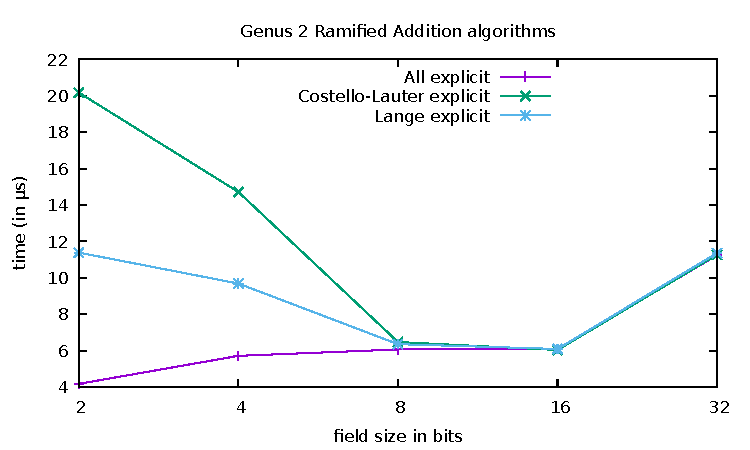
\includegraphics[width=0.775\textwidth]{genus2/g2_G1_RAM_ADD.pdf}}
\centerline{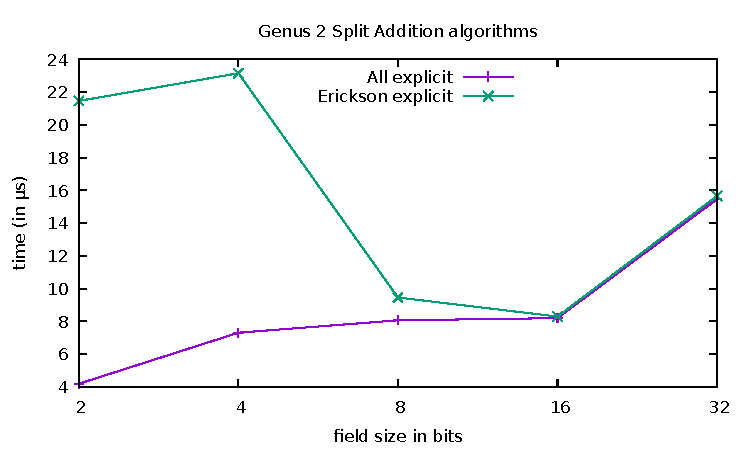
\includegraphics[width=0.775\textwidth]{genus2/g2_G1_SPL_ADD.pdf}}

\subsection{Ramified and Split Model Comparisons}

In the next figures, explicit formulas introduced in this work are compared to
all relevant previous best algorithms over ramified and split models. Our split
and ramified model formulas are also plotted for comparison of genus 2
arithmetic in the last figure. The following conclusions are drawn from these plots:
\begin{itemize}
    \item On the same platform, our explicit formulas outperform all relevant
    previous algorithms, including state-of-the-art and Cantor based algorithms,
    over every field size.

    \item Expensive field multiplication for addition trades, such as the trade
    of 13 additions for 1 multiplication proposed
    in~\cite{CostelloLauter_geo_2011} are detrimental for efficiency over any
    field size, providing evidence for the design choices of this work to cap
    trades at 3 additions for 1 multiplication (see Section~\ref{sec:trades}).
     
    \item Our explicit formulas outperform Magma's built-in arithmetic over
    512-bit fields and up for ramified models and 1024-bit fields for split
    models. Based on the relative performance of prior state-of-the-art, Magma
    is likely accessing internal $C$ functions that is not accessible via the
    interface provided.

    \item For Magma based implementations, split model arithmetic using balanced
    divisor classes is about $20\%$ slower than ramified arithmetic for genus 2
    curves. 
\end{itemize}

\centerline{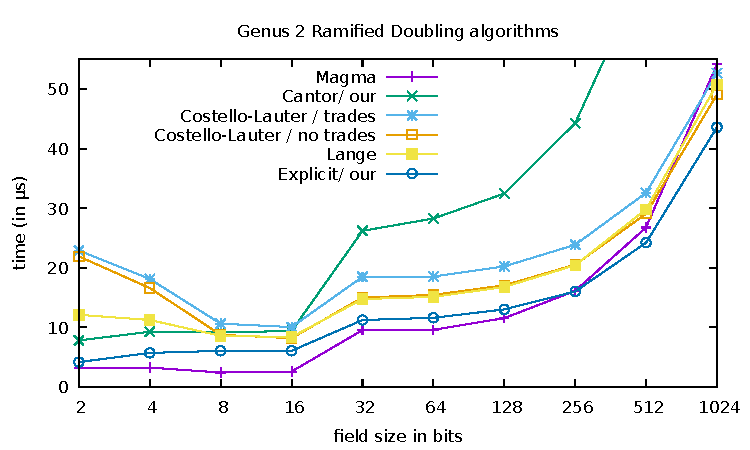
\includegraphics[width=0.775\textwidth]{genus2/g2_G2_RAM_ADD.pdf}}
\centerline{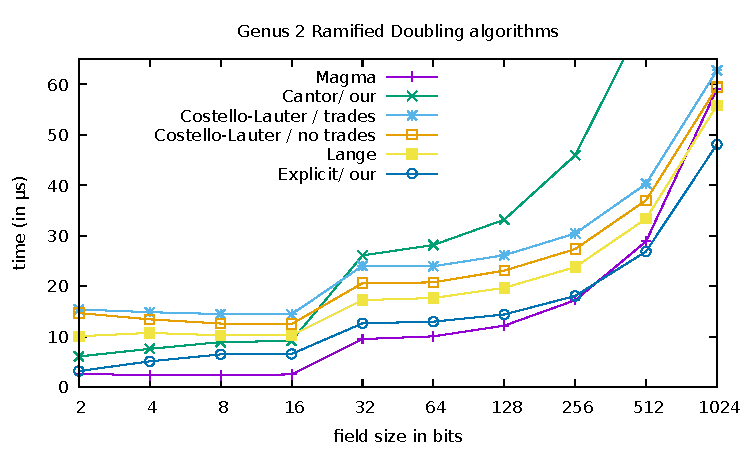
\includegraphics[width=0.775\textwidth]{genus2/g2_G2_RAM_DBL.pdf}}
\centerline{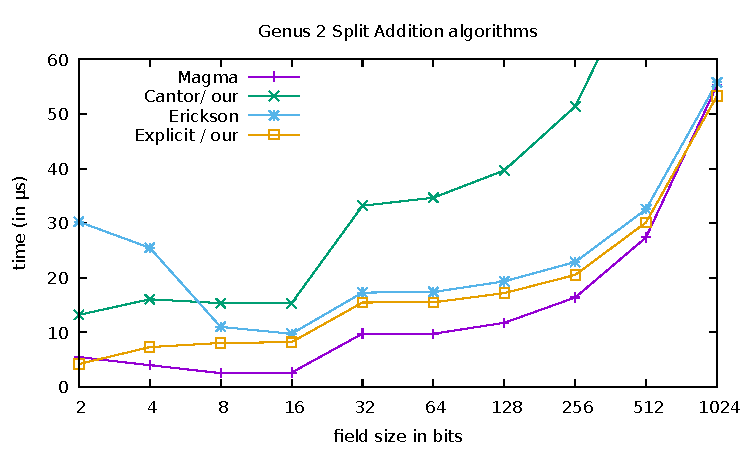
\includegraphics[width=0.775\textwidth]{genus2/g2_G3_SPL_ADD.pdf}}
\centerline{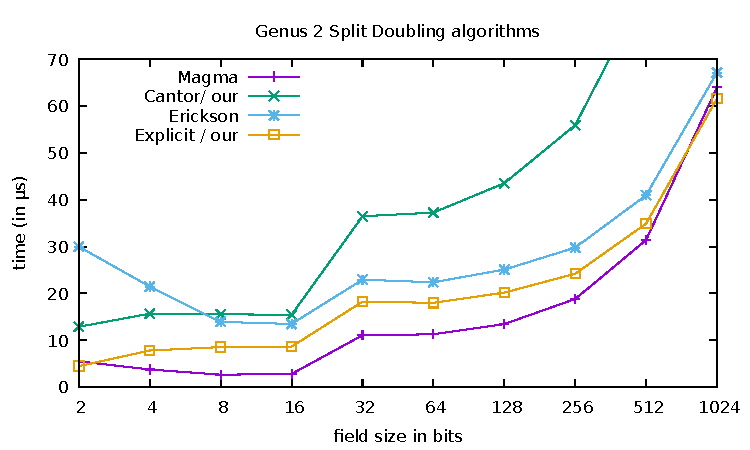
\includegraphics[width=0.775\textwidth]{genus2/g2_G3_SPL_DBL.pdf}}
\centerline{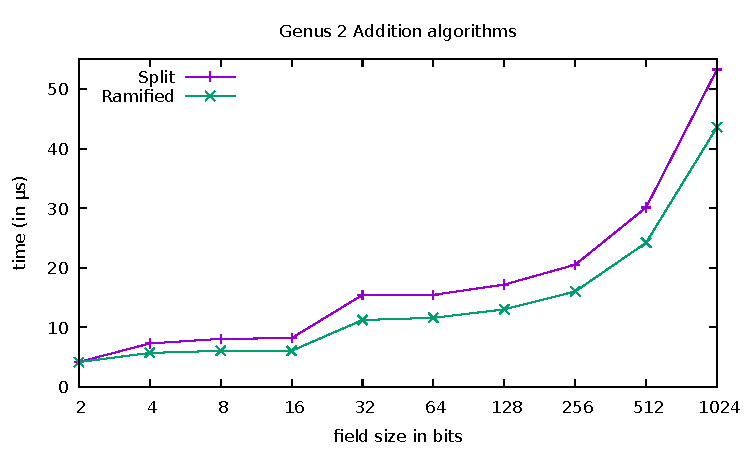
\includegraphics[width=0.775\textwidth]{genus2/g2_G4_ADD.pdf}}
\centerline{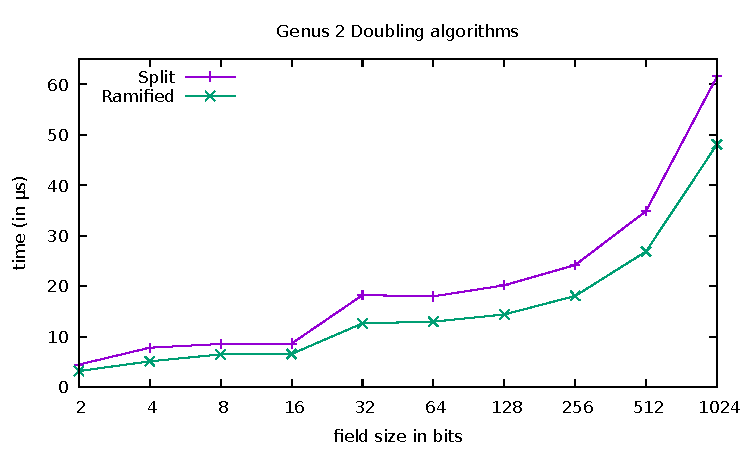
\includegraphics[width=0.775\textwidth]{genus2/g2_G4_DBL.pdf}}

\subsection{Summary}

The empirical results indicate that complete explicit formulas provide an
improvement for computing ramified and split model arithmetic over small
cardinality fields with a cross-over at 16-bits.  As expected, the relatively
fewer field operations required in the formulas of this work translate to faster
implementations when using the same platform. The relative performance of
Magma's built-in arithmetic and the formulas of this chapter is likely due to
Magma's high-level interface. Integrating algorithms from this chapter directly
into Magma's built-in arithmetic, or implementing the algorithms directly in
C/C++ so that they do not suffer from the overhead associated to working in a
high-level system like Magma, should reduce the relative performance to Magma's
built-in arithmetic, the relative performance between genus 2 split and ramified
model arithmetic and increase the field size for performance convergence between
complete explicit formulas and frequent case only implementations.




